\documentclass[11pt,a4paper]{article}
\usepackage[utf8]{inputenc}
\usepackage[T1]{fontenc}
\usepackage{geometry}
\usepackage{booktabs}
\usepackage{longtable}
\usepackage{array}
\usepackage{graphicx}
\usepackage{xcolor}
\usepackage{hyperref}
\usepackage{amsmath}
\usepackage{siunitx}
\usepackage{adjustbox}
\usepackage{pgfplots}
\usepackage{tikz}
\usepackage{pdflscape}
\usepackage{url}
\pgfplotsset{compat=1.18}

\geometry{margin=1in}
\hypersetup{
    colorlinks=true,
    linkcolor=blue,
    filecolor=magenta,      
    urlcolor=cyan,
}

\title{Window Size Analysis Report\\
\large Cross-Validation Results for Behavior Classification}
\author{Automated Analysis Pipeline}
\date{\today}

\definecolor{bestgreen}{RGB}{39, 174, 96}
\definecolor{bestred}{RGB}{231, 76, 60}
\definecolor{infoblue}{RGB}{52, 152, 219}

\begin{document}

\maketitle

\begin{abstract}
This report presents a comprehensive analysis of window size effects on behavior classification performance using leave-one-out cross-validation. The analysis examines performance metrics across multiple window sizes (5, 10, 15, 20, 30 frames) to identify the optimal temporal scale for feature generation and classification. Key findings include the identification of Window 30 frames as the optimal window size, with a mean accuracy of 0.9031 and F1 (Behavior) score of 0.8087. The analysis also identifies worst-performing videos that may require data quality review and window-sensitive videos that show high variability across temporal scales. A total of 52 unique videos were analyzed across 5 window sizes, representing 305 individual test cases.
\end{abstract}

\tableofcontents
\newpage

\section{Introduction}

\subsection{Purpose and Scope}

This analysis examines the effect of window size on behavior classification performance for the \textit{turn\_left} behavior. Window size is a critical hyperparameter in temporal feature extraction, as it determines the temporal scale at which behavioral patterns are captured. Too small a window may miss important behavioral dynamics, while too large a window may introduce noise or blur important short-term patterns.

The analysis compares performance across window sizes of 5, 10, 15, 20, 30 frames, using leave-one-out cross-validation where one animal (identity) is held out at a time. This approach ensures robust performance estimates while maintaining independence between training and test sets.

\subsection{Data Structure}

The cross-validation structure used in this analysis holds out \textbf{one animal at a time}, not one video at a time. Each video file contains multiple animals, identified by identity numbers [0], [1], [2], etc. at the end of the video filename. This means that the same video file appears multiple times in the results, each time representing a different animal being held out during cross-validation. Each (video\_name, identity) pair represents a separate test case, ensuring that the model's performance is evaluated independently for each animal.

\subsection{Performance Metrics}

The analysis focuses on several key performance metrics:

\begin{itemize}
    \item \textbf{Accuracy}: Overall classification accuracy across both behavior and not-behavior classes
    \item \textbf{F1 (Behavior)}: F1 score for the behavior class - the most relevant metric for behavior classification, as it balances precision and recall for the class of interest
    \item \textbf{F1 (Not Behavior)}: F1 score for the not-behavior class
    \item \textbf{Precision and Recall}: Class-specific precision and recall for both classes
\end{itemize}

Of these metrics, \textbf{F1 (Behavior)} is considered the most relevant for this analysis, as it directly measures the model's ability to correctly identify the behavior of interest while accounting for both false positives and false negatives.

\section{Executive Summary}

\subsection{Key Findings}

The analysis reveals that \textbf{Window 30 frames} provides the optimal balance between classification performance and stability. This window size achieves:

\begin{itemize}
    \item Mean accuracy of 0.9031
    \item Mean F1 (Behavior) of 0.8087 (most relevant metric)
    \item Standard deviation of 0.0882 for accuracy, indicating good stability
    \item Standard deviation of 0.1870 for F1 (Behavior)
\end{itemize}

\subsection{Performance Trends}

Several important trends emerge from the analysis:

\begin{enumerate}
    \item \textbf{Larger windows generally perform better}: Window sizes of 20-30 frames show significantly higher accuracy and F1 (Behavior) scores than smaller windows (5-10 frames). This suggests that the \textit{turn\_left} behavior benefits from a longer temporal context for accurate classification.
    
    \item \textbf{Performance plateau}: There is minimal difference between Window 20 and Window 30 frames (difference in accuracy: 0.0000), suggesting that beyond 20 frames, additional temporal context provides diminishing returns.
    
    \item \textbf{Window 5 frames shows lowest performance}: With mean accuracy of 0.8234 and F1 (Behavior) of 0.7249, the smallest window size is insufficient for capturing the behavioral dynamics of \textit{turn\_left}.
    
    \item \textbf{Stability considerations}: Window 20 frames shows slightly better stability (lower standard deviation) than Window 30 frames, making it preferable when consistency is important.
\end{enumerate}

\section{Window Size Comparison}

\subsection{Overall Performance Metrics}

Table~\ref{tab:window_comparison} presents a comprehensive comparison of performance metrics across all tested window sizes. The table includes mean and standard deviation for accuracy and F1 scores for both behavior and not-behavior classes.

\begin{table}[h]
\centering
\caption{Performance Summary by Window Size}
\label{tab:window_comparison}
\adjustbox{width=\textwidth,center}{%
\begin{tabular}{lcccccc}
\toprule
Window Size & Mean Acc. & SD Acc. & Mean F1 (Beh.) & SD F1 (Beh.) & Mean F1 (Not) & SD F1 (Not) \\
\midrule
5 & 0.8234 & 0.0947 & 0.7249 & 0.1356 & 0.8475 & 0.1118 \\
10 & 0.8717 & 0.1023 & 0.7926 & 0.1457 & 0.8818 & 0.1368 \\
15 & 0.8927 & 0.0854 & 0.8073 & 0.1749 & 0.9094 & 0.0843 \\
20 & 0.9026 & 0.0890 & \textcolor{bestred}{\textbf{0.8214}} & 0.1620 & 0.9170 & 0.0988 \\
30 & \textcolor{bestgreen}{\textbf{0.9031}} & 0.0882 & 0.8087 & 0.1870 & 0.9225 & 0.0829 \\
\bottomrule
\end{tabular}
\endadjustbox
\end{table}

\subsection{Visualization of Performance Metrics}

The following plots visualize the performance metrics across different window sizes, highlighting the best performing window for each metric.


\begin{figure}[h]
\centering

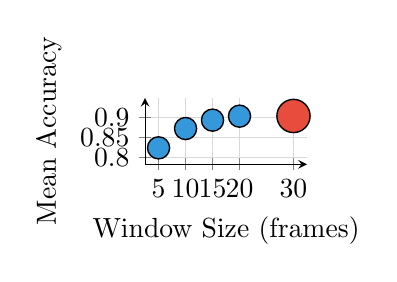
\begin{tikzpicture}
\begin{axis}[
    width=0.3\textwidth,
    height=0.2\textwidth,
    ymin=0.7822,
    ymax=0.9483,
    xlabel={Window Size (frames)},
    ylabel={Mean Accuracy},
    xtick={5,10,15,20,30},
    xticklabels={5,10,15,20,30},
    grid=major,
    grid style={gray!30},
    axis lines=left,
    enlarge x limits=0.1,
]
\addplot[only marks, mark=*, mark size=4pt, fill=infoblue, draw=black, line width=0.5pt] coordinates {(5, 0.8234)};
\addplot[only marks, mark=*, mark size=4pt, fill=infoblue, draw=black, line width=0.5pt] coordinates {(10, 0.8717)};
\addplot[only marks, mark=*, mark size=4pt, fill=infoblue, draw=black, line width=0.5pt] coordinates {(15, 0.8927)};
\addplot[only marks, mark=*, mark size=4pt, fill=infoblue, draw=black, line width=0.5pt] coordinates {(20, 0.9026)};
\addplot[only marks, mark=*, mark size=6pt, fill=bestred, draw=black, line width=0.5pt] coordinates {(30, 0.9031)};

\end{axis}
\end{tikzpicture}

\caption{Mean Accuracy by Window Size}
\label{fig:mean_accuracy}
\end{figure}

\begin{figure}[h]
\centering

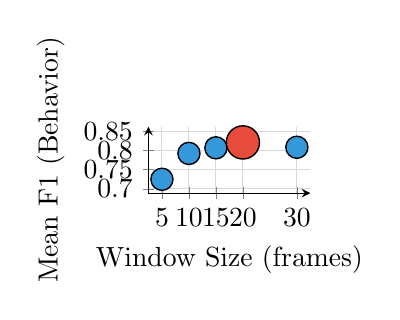
\begin{tikzpicture}
\begin{axis}[
    width=0.3\textwidth,
    height=0.2\textwidth,
    ymin=0.6886,
    ymax=0.8625,
    xlabel={Window Size (frames)},
    ylabel={Mean F1 (Behavior)},
    xtick={5,10,15,20,30},
    xticklabels={5,10,15,20,30},
    grid=major,
    grid style={gray!30},
    axis lines=left,
    enlarge x limits=0.1,
]
\addplot[only marks, mark=*, mark size=4pt, fill=infoblue, draw=black, line width=0.5pt] coordinates {(5, 0.7249)};
\addplot[only marks, mark=*, mark size=4pt, fill=infoblue, draw=black, line width=0.5pt] coordinates {(10, 0.7926)};
\addplot[only marks, mark=*, mark size=4pt, fill=infoblue, draw=black, line width=0.5pt] coordinates {(15, 0.8073)};
\addplot[only marks, mark=*, mark size=6pt, fill=bestred, draw=black, line width=0.5pt] coordinates {(20, 0.8214)};
\addplot[only marks, mark=*, mark size=4pt, fill=infoblue, draw=black, line width=0.5pt] coordinates {(30, 0.8087)};

\end{axis}
\end{tikzpicture}

\caption{Mean F1 (Behavior) by Window Size}
\label{fig:mean_f1_behavior}
\end{figure}

\begin{figure}[h]
\centering

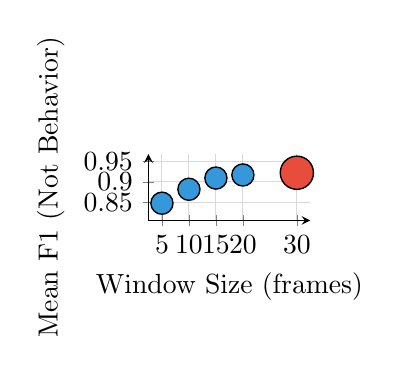
\begin{tikzpicture}
\begin{axis}[
    width=0.3\textwidth,
    height=0.2\textwidth,
    ymin=0.8051,
    ymax=0.9686,
    xlabel={Window Size (frames)},
    ylabel={Mean F1 (Not Behavior)},
    xtick={5,10,15,20,30},
    xticklabels={5,10,15,20,30},
    grid=major,
    grid style={gray!30},
    axis lines=left,
    enlarge x limits=0.1,
]
\addplot[only marks, mark=*, mark size=4pt, fill=infoblue, draw=black, line width=0.5pt] coordinates {(5, 0.8475)};
\addplot[only marks, mark=*, mark size=4pt, fill=infoblue, draw=black, line width=0.5pt] coordinates {(10, 0.8818)};
\addplot[only marks, mark=*, mark size=4pt, fill=infoblue, draw=black, line width=0.5pt] coordinates {(15, 0.9094)};
\addplot[only marks, mark=*, mark size=4pt, fill=infoblue, draw=black, line width=0.5pt] coordinates {(20, 0.9170)};
\addplot[only marks, mark=*, mark size=6pt, fill=bestred, draw=black, line width=0.5pt] coordinates {(30, 0.9225)};

\end{axis}
\end{tikzpicture}

\caption{Mean F1 (Not Behavior) by Window Size}
\label{fig:mean_f1_notbeh}
\end{figure}

\subsection{Interpretation of Results}

The results in Table~\ref{tab:window_comparison} reveal several important patterns. Window 30 frames achieves the highest mean accuracy of 0.9031, while Window 20 frames achieves the highest F1 (Behavior) score of 0.8214. 

Since F1 (Behavior) is the most relevant metric for behavior classification, Window 20 frames is recommended as the optimal choice. This metric balances precision and recall for the behavior class, which is critical when the goal is to accurately identify instances of the target behavior.

The standard deviations provide insight into the stability of each window size. Lower standard deviations indicate more consistent performance across videos, which is desirable for reliable classification. Window 30 frames shows good stability with a standard deviation of 0.0882 for accuracy.

\section{Per-Video Performance Distribution}

\subsection{Distribution Analysis}

To understand the variability in performance across different videos, we examine the distribution of performance metrics for each window size. This analysis helps identify whether performance differences are consistent across all videos or if certain videos drive the observed patterns.

\subsection{Accuracy Distribution}

The accuracy distribution across all videos for each window size shows that:

\begin{itemize}
    \item Window 30 frames has the highest median accuracy
    \item The interquartile range (IQR) is narrower for larger windows, indicating more consistent performance
    \item Outliers are more common in smaller window sizes, suggesting that some videos are particularly sensitive to insufficient temporal context
\end{itemize}

The following box-whisker plots show individual video performance as points, with outliers highlighted. This visualization reveals that while most videos perform well with Window 30 frames, a small number of videos show poor performance regardless of window size, suggesting potential data quality issues.


\begin{figure}[h]
\centering

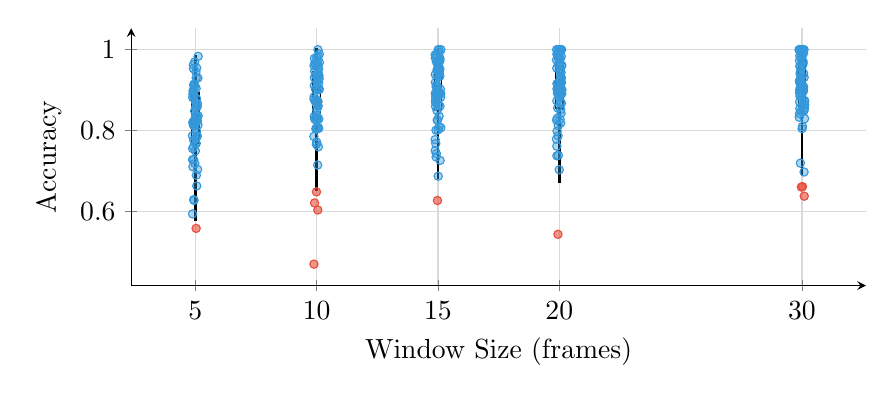
\begin{tikzpicture}
\begin{axis}[
    width=0.9\textwidth,
    height=0.4\textwidth,
    ymin=0.4176,
    ymax=1.0529,
    xlabel={Window Size (frames)},
    ylabel={Accuracy},
    xtick={5,10,15,20,30},
    xticklabels={5,10,15,20,30},
    grid=major,
    grid style={gray!30},
    axis lines=left,
    enlarge x limits=0.1,
]
\draw[fill=infoblue!30, draw=black, line width=0.5pt] (axis cs:4.850,0.7688) rectangle (axis cs:5.150,0.8947);
\draw[draw=black, line width=1.5pt] (axis cs:4.850,0.8333) -- (axis cs:5.150,0.8333);
\draw[draw=black, line width=1pt] (axis cs:5.000,0.5799) -- (axis cs:5.000,0.7688);
\draw[draw=black, line width=1pt] (axis cs:5.000,0.8947) -- (axis cs:5.000,0.9835);
\draw[draw=black, line width=1pt] (axis cs:4.940,0.5799) -- (axis cs:5.060,0.5799);
\draw[draw=black, line width=1pt] (axis cs:4.940,0.9835) -- (axis cs:5.060,0.9835);
\addplot[only marks, mark=*, mark size=2pt, color=gray, fill=gray] coordinates {(5.000, 0.8234)};
\addplot[only marks, mark=*, mark size=1.5pt, color=bestred, fill=bestred, fill opacity=0.6] coordinates {(5.033, 0.5588)};
\addplot[only marks, mark=*, mark size=1.5pt, color=infoblue, fill=infoblue, fill opacity=0.4] coordinates {(4.886, 0.5946)};
\addplot[only marks, mark=*, mark size=1.5pt, color=infoblue, fill=infoblue, fill opacity=0.4] coordinates {(4.946, 0.6279)};
\addplot[only marks, mark=*, mark size=1.5pt, color=infoblue, fill=infoblue, fill opacity=0.4] coordinates {(4.934, 0.6296)};
\addplot[only marks, mark=*, mark size=1.5pt, color=infoblue, fill=infoblue, fill opacity=0.4] coordinates {(5.057, 0.6636)};
\addplot[only marks, mark=*, mark size=1.5pt, color=infoblue, fill=infoblue, fill opacity=0.4] coordinates {(5.042, 0.6901)};
\addplot[only marks, mark=*, mark size=1.5pt, color=infoblue, fill=infoblue, fill opacity=0.4] coordinates {(5.094, 0.7043)};
\addplot[only marks, mark=*, mark size=1.5pt, color=infoblue, fill=infoblue, fill opacity=0.4] coordinates {(4.901, 0.7108)};
\addplot[only marks, mark=*, mark size=1.5pt, color=infoblue, fill=infoblue, fill opacity=0.4] coordinates {(4.981, 0.7190)};
\addplot[only marks, mark=*, mark size=1.5pt, color=infoblue, fill=infoblue, fill opacity=0.4] coordinates {(4.887, 0.7283)};
\addplot[only marks, mark=*, mark size=1.5pt, color=infoblue, fill=infoblue, fill opacity=0.4] coordinates {(4.932, 0.7284)};
\addplot[only marks, mark=*, mark size=1.5pt, color=infoblue, fill=infoblue, fill opacity=0.4] coordinates {(5.001, 0.7500)};
\addplot[only marks, mark=*, mark size=1.5pt, color=infoblue, fill=infoblue, fill opacity=0.4] coordinates {(4.886, 0.7558)};
\addplot[only marks, mark=*, mark size=1.5pt, color=infoblue, fill=infoblue, fill opacity=0.4] coordinates {(4.928, 0.7603)};
\addplot[only marks, mark=*, mark size=1.5pt, color=infoblue, fill=infoblue, fill opacity=0.4] coordinates {(5.036, 0.7684)};
\addplot[only marks, mark=*, mark size=1.5pt, color=infoblue, fill=infoblue, fill opacity=0.4] coordinates {(5.011, 0.7688)};
\addplot[only marks, mark=*, mark size=1.5pt, color=infoblue, fill=infoblue, fill opacity=0.4] coordinates {(4.933, 0.7764)};
\addplot[only marks, mark=*, mark size=1.5pt, color=infoblue, fill=infoblue, fill opacity=0.4] coordinates {(5.021, 0.7805)};
\addplot[only marks, mark=*, mark size=1.5pt, color=infoblue, fill=infoblue, fill opacity=0.4] coordinates {(5.074, 0.7857)};
\addplot[only marks, mark=*, mark size=1.5pt, color=infoblue, fill=infoblue, fill opacity=0.4] coordinates {(4.882, 0.7872)};
\addplot[only marks, mark=*, mark size=1.5pt, color=infoblue, fill=infoblue, fill opacity=0.4] coordinates {(5.073, 0.7880)};
\addplot[only marks, mark=*, mark size=1.5pt, color=infoblue, fill=infoblue, fill opacity=0.4] coordinates {(5.048, 0.7987)};
\addplot[only marks, mark=*, mark size=1.5pt, color=infoblue, fill=infoblue, fill opacity=0.4] coordinates {(4.962, 0.8108)};
\addplot[only marks, mark=*, mark size=1.5pt, color=infoblue, fill=infoblue, fill opacity=0.4] coordinates {(4.917, 0.8140)};
\addplot[only marks, mark=*, mark size=1.5pt, color=infoblue, fill=infoblue, fill opacity=0.4] coordinates {(5.110, 0.8140)};
\addplot[only marks, mark=*, mark size=1.5pt, color=infoblue, fill=infoblue, fill opacity=0.4] coordinates {(4.961, 0.8170)};
\addplot[only marks, mark=*, mark size=1.5pt, color=infoblue, fill=infoblue, fill opacity=0.4] coordinates {(4.902, 0.8194)};
\addplot[only marks, mark=*, mark size=1.5pt, color=infoblue, fill=infoblue, fill opacity=0.4] coordinates {(4.903, 0.8212)};
\addplot[only marks, mark=*, mark size=1.5pt, color=infoblue, fill=infoblue, fill opacity=0.4] coordinates {(5.083, 0.8250)};
\addplot[only marks, mark=*, mark size=1.5pt, color=infoblue, fill=infoblue, fill opacity=0.4] coordinates {(5.025, 0.8261)};
\addplot[only marks, mark=*, mark size=1.5pt, color=infoblue, fill=infoblue, fill opacity=0.4] coordinates {(5.074, 0.8333)};
\addplot[only marks, mark=*, mark size=1.5pt, color=infoblue, fill=infoblue, fill opacity=0.4] coordinates {(5.055, 0.8356)};
\addplot[only marks, mark=*, mark size=1.5pt, color=infoblue, fill=infoblue, fill opacity=0.4] coordinates {(5.009, 0.8359)};
\addplot[only marks, mark=*, mark size=1.5pt, color=infoblue, fill=infoblue, fill opacity=0.4] coordinates {(5.114, 0.8367)};
\addplot[only marks, mark=*, mark size=1.5pt, color=infoblue, fill=infoblue, fill opacity=0.4] coordinates {(4.971, 0.8485)};
\addplot[only marks, mark=*, mark size=1.5pt, color=infoblue, fill=infoblue, fill opacity=0.4] coordinates {(5.012, 0.8560)};
\addplot[only marks, mark=*, mark size=1.5pt, color=infoblue, fill=infoblue, fill opacity=0.4] coordinates {(5.079, 0.8595)};
\addplot[only marks, mark=*, mark size=1.5pt, color=infoblue, fill=infoblue, fill opacity=0.4] coordinates {(5.028, 0.8607)};
\addplot[only marks, mark=*, mark size=1.5pt, color=infoblue, fill=infoblue, fill opacity=0.4] coordinates {(5.087, 0.8667)};
\addplot[only marks, mark=*, mark size=1.5pt, color=infoblue, fill=infoblue, fill opacity=0.4] coordinates {(5.019, 0.8691)};
\addplot[only marks, mark=*, mark size=1.5pt, color=infoblue, fill=infoblue, fill opacity=0.4] coordinates {(5.049, 0.8791)};
\addplot[only marks, mark=*, mark size=1.5pt, color=infoblue, fill=infoblue, fill opacity=0.4] coordinates {(4.891, 0.8816)};
\addplot[only marks, mark=*, mark size=1.5pt, color=infoblue, fill=infoblue, fill opacity=0.4] coordinates {(4.935, 0.8848)};
\addplot[only marks, mark=*, mark size=1.5pt, color=infoblue, fill=infoblue, fill opacity=0.4] coordinates {(4.949, 0.8869)};
\addplot[only marks, mark=*, mark size=1.5pt, color=infoblue, fill=infoblue, fill opacity=0.4] coordinates {(4.899, 0.8904)};
\addplot[only marks, mark=*, mark size=1.5pt, color=infoblue, fill=infoblue, fill opacity=0.4] coordinates {(4.936, 0.8947)};
\addplot[only marks, mark=*, mark size=1.5pt, color=infoblue, fill=infoblue, fill opacity=0.4] coordinates {(4.904, 0.8981)};
\addplot[only marks, mark=*, mark size=1.5pt, color=infoblue, fill=infoblue, fill opacity=0.4] coordinates {(4.947, 0.9032)};
\addplot[only marks, mark=*, mark size=1.5pt, color=infoblue, fill=infoblue, fill opacity=0.4] coordinates {(5.033, 0.9045)};
\addplot[only marks, mark=*, mark size=1.5pt, color=infoblue, fill=infoblue, fill opacity=0.4] coordinates {(4.968, 0.9109)};
\addplot[only marks, mark=*, mark size=1.5pt, color=infoblue, fill=infoblue, fill opacity=0.4] coordinates {(4.969, 0.9121)};
\addplot[only marks, mark=*, mark size=1.5pt, color=infoblue, fill=infoblue, fill opacity=0.4] coordinates {(4.930, 0.9124)};
\addplot[only marks, mark=*, mark size=1.5pt, color=infoblue, fill=infoblue, fill opacity=0.4] coordinates {(4.944, 0.9148)};
\addplot[only marks, mark=*, mark size=1.5pt, color=infoblue, fill=infoblue, fill opacity=0.4] coordinates {(5.105, 0.9299)};
\addplot[only marks, mark=*, mark size=1.5pt, color=infoblue, fill=infoblue, fill opacity=0.4] coordinates {(5.036, 0.9304)};
\addplot[only marks, mark=*, mark size=1.5pt, color=infoblue, fill=infoblue, fill opacity=0.4] coordinates {(5.026, 0.9448)};
\addplot[only marks, mark=*, mark size=1.5pt, color=infoblue, fill=infoblue, fill opacity=0.4] coordinates {(4.921, 0.9533)};
\addplot[only marks, mark=*, mark size=1.5pt, color=infoblue, fill=infoblue, fill opacity=0.4] coordinates {(5.055, 0.9547)};
\addplot[only marks, mark=*, mark size=1.5pt, color=infoblue, fill=infoblue, fill opacity=0.4] coordinates {(4.919, 0.9626)};
\addplot[only marks, mark=*, mark size=1.5pt, color=infoblue, fill=infoblue, fill opacity=0.4] coordinates {(4.971, 0.9695)};
\addplot[only marks, mark=*, mark size=1.5pt, color=infoblue, fill=infoblue, fill opacity=0.4] coordinates {(5.117, 0.9835)};
\draw[fill=infoblue!30, draw=black, line width=0.5pt] (axis cs:9.850,0.8286) rectangle (axis cs:10.150,0.9446);
\draw[draw=black, line width=1.5pt] (axis cs:9.850,0.9020) -- (axis cs:10.150,0.9020);
\draw[draw=black, line width=1pt] (axis cs:10.000,0.6545) -- (axis cs:10.000,0.8286);
\draw[draw=black, line width=1pt] (axis cs:10.000,0.9446) -- (axis cs:10.000,1.0000);
\draw[draw=black, line width=1pt] (axis cs:9.940,0.6545) -- (axis cs:10.060,0.6545);
\draw[draw=black, line width=1pt] (axis cs:9.940,1.0000) -- (axis cs:10.060,1.0000);
\addplot[only marks, mark=*, mark size=2pt, color=gray, fill=gray] coordinates {(10.000, 0.8717)};
\addplot[only marks, mark=*, mark size=1.5pt, color=bestred, fill=bestred, fill opacity=0.6] coordinates {(9.889, 0.4706)};
\addplot[only marks, mark=*, mark size=1.5pt, color=bestred, fill=bestred, fill opacity=0.6] coordinates {(10.047, 0.6042)};
\addplot[only marks, mark=*, mark size=1.5pt, color=bestred, fill=bestred, fill opacity=0.6] coordinates {(9.915, 0.6216)};
\addplot[only marks, mark=*, mark size=1.5pt, color=bestred, fill=bestred, fill opacity=0.6] coordinates {(9.991, 0.6489)};
\addplot[only marks, mark=*, mark size=1.5pt, color=infoblue, fill=infoblue, fill opacity=0.4] coordinates {(10.041, 0.7151)};
\addplot[only marks, mark=*, mark size=1.5pt, color=infoblue, fill=infoblue, fill opacity=0.4] coordinates {(10.070, 0.7602)};
\addplot[only marks, mark=*, mark size=1.5pt, color=infoblue, fill=infoblue, fill opacity=0.4] coordinates {(9.989, 0.7664)};
\addplot[only marks, mark=*, mark size=1.5pt, color=infoblue, fill=infoblue, fill opacity=0.4] coordinates {(10.000, 0.7717)};
\addplot[only marks, mark=*, mark size=1.5pt, color=infoblue, fill=infoblue, fill opacity=0.4] coordinates {(9.885, 0.7857)};
\addplot[only marks, mark=*, mark size=1.5pt, color=infoblue, fill=infoblue, fill opacity=0.4] coordinates {(9.984, 0.8046)};
\addplot[only marks, mark=*, mark size=1.5pt, color=infoblue, fill=infoblue, fill opacity=0.4] coordinates {(9.969, 0.8051)};
\addplot[only marks, mark=*, mark size=1.5pt, color=infoblue, fill=infoblue, fill opacity=0.4] coordinates {(10.085, 0.8056)};
\addplot[only marks, mark=*, mark size=1.5pt, color=infoblue, fill=infoblue, fill opacity=0.4] coordinates {(10.011, 0.8079)};
\addplot[only marks, mark=*, mark size=1.5pt, color=infoblue, fill=infoblue, fill opacity=0.4] coordinates {(10.061, 0.8083)};
\addplot[only marks, mark=*, mark size=1.5pt, color=infoblue, fill=infoblue, fill opacity=0.4] coordinates {(9.984, 0.8256)};
\addplot[only marks, mark=*, mark size=1.5pt, color=infoblue, fill=infoblue, fill opacity=0.4] coordinates {(9.922, 0.8286)};
\addplot[only marks, mark=*, mark size=1.5pt, color=infoblue, fill=infoblue, fill opacity=0.4] coordinates {(10.084, 0.8288)};
\addplot[only marks, mark=*, mark size=1.5pt, color=infoblue, fill=infoblue, fill opacity=0.4] coordinates {(10.077, 0.8293)};
\addplot[only marks, mark=*, mark size=1.5pt, color=infoblue, fill=infoblue, fill opacity=0.4] coordinates {(9.970, 0.8321)};
\addplot[only marks, mark=*, mark size=1.5pt, color=infoblue, fill=infoblue, fill opacity=0.4] coordinates {(9.903, 0.8352)};
\addplot[only marks, mark=*, mark size=1.5pt, color=infoblue, fill=infoblue, fill opacity=0.4] coordinates {(10.003, 0.8387)};
\addplot[only marks, mark=*, mark size=1.5pt, color=infoblue, fill=infoblue, fill opacity=0.4] coordinates {(9.999, 0.8515)};
\addplot[only marks, mark=*, mark size=1.5pt, color=infoblue, fill=infoblue, fill opacity=0.4] coordinates {(10.065, 0.8609)};
\addplot[only marks, mark=*, mark size=1.5pt, color=infoblue, fill=infoblue, fill opacity=0.4] coordinates {(10.023, 0.8641)};
\addplot[only marks, mark=*, mark size=1.5pt, color=infoblue, fill=infoblue, fill opacity=0.4] coordinates {(10.002, 0.8649)};
\addplot[only marks, mark=*, mark size=1.5pt, color=infoblue, fill=infoblue, fill opacity=0.4] coordinates {(10.018, 0.8737)};
\addplot[only marks, mark=*, mark size=1.5pt, color=infoblue, fill=infoblue, fill opacity=0.4] coordinates {(9.970, 0.8760)};
\addplot[only marks, mark=*, mark size=1.5pt, color=infoblue, fill=infoblue, fill opacity=0.4] coordinates {(9.892, 0.8776)};
\addplot[only marks, mark=*, mark size=1.5pt, color=infoblue, fill=infoblue, fill opacity=0.4] coordinates {(9.895, 0.8833)};
\addplot[only marks, mark=*, mark size=1.5pt, color=infoblue, fill=infoblue, fill opacity=0.4] coordinates {(10.106, 0.9015)};
\addplot[only marks, mark=*, mark size=1.5pt, color=infoblue, fill=infoblue, fill opacity=0.4] coordinates {(10.081, 0.9020)};
\addplot[only marks, mark=*, mark size=1.5pt, color=infoblue, fill=infoblue, fill opacity=0.4] coordinates {(9.951, 0.9026)};
\addplot[only marks, mark=*, mark size=1.5pt, color=infoblue, fill=infoblue, fill opacity=0.4] coordinates {(10.093, 0.9041)};
\addplot[only marks, mark=*, mark size=1.5pt, color=infoblue, fill=infoblue, fill opacity=0.4] coordinates {(10.005, 0.9070)};
\addplot[only marks, mark=*, mark size=1.5pt, color=infoblue, fill=infoblue, fill opacity=0.4] coordinates {(9.905, 0.9114)};
\addplot[only marks, mark=*, mark size=1.5pt, color=infoblue, fill=infoblue, fill opacity=0.4] coordinates {(10.085, 0.9178)};
\addplot[only marks, mark=*, mark size=1.5pt, color=infoblue, fill=infoblue, fill opacity=0.4] coordinates {(10.020, 0.9197)};
\addplot[only marks, mark=*, mark size=1.5pt, color=infoblue, fill=infoblue, fill opacity=0.4] coordinates {(10.104, 0.9286)};
\addplot[only marks, mark=*, mark size=1.5pt, color=infoblue, fill=infoblue, fill opacity=0.4] coordinates {(10.043, 0.9306)};
\addplot[only marks, mark=*, mark size=1.5pt, color=infoblue, fill=infoblue, fill opacity=0.4] coordinates {(9.903, 0.9307)};
\addplot[only marks, mark=*, mark size=1.5pt, color=infoblue, fill=infoblue, fill opacity=0.4] coordinates {(10.029, 0.9356)};
\addplot[only marks, mark=*, mark size=1.5pt, color=infoblue, fill=infoblue, fill opacity=0.4] coordinates {(10.069, 0.9357)};
\addplot[only marks, mark=*, mark size=1.5pt, color=infoblue, fill=infoblue, fill opacity=0.4] coordinates {(10.096, 0.9360)};
\addplot[only marks, mark=*, mark size=1.5pt, color=infoblue, fill=infoblue, fill opacity=0.4] coordinates {(9.960, 0.9367)};
\addplot[only marks, mark=*, mark size=1.5pt, color=infoblue, fill=infoblue, fill opacity=0.4] coordinates {(10.007, 0.9391)};
\addplot[only marks, mark=*, mark size=1.5pt, color=infoblue, fill=infoblue, fill opacity=0.4] coordinates {(10.048, 0.9446)};
\addplot[only marks, mark=*, mark size=1.5pt, color=infoblue, fill=infoblue, fill opacity=0.4] coordinates {(9.920, 0.9466)};
\addplot[only marks, mark=*, mark size=1.5pt, color=infoblue, fill=infoblue, fill opacity=0.4] coordinates {(10.084, 0.9529)};
\addplot[only marks, mark=*, mark size=1.5pt, color=infoblue, fill=infoblue, fill opacity=0.4] coordinates {(10.067, 0.9545)};
\addplot[only marks, mark=*, mark size=1.5pt, color=infoblue, fill=infoblue, fill opacity=0.4] coordinates {(9.892, 0.9605)};
\addplot[only marks, mark=*, mark size=1.5pt, color=infoblue, fill=infoblue, fill opacity=0.4] coordinates {(10.022, 0.9609)};
\addplot[only marks, mark=*, mark size=1.5pt, color=infoblue, fill=infoblue, fill opacity=0.4] coordinates {(9.968, 0.9621)};
\addplot[only marks, mark=*, mark size=1.5pt, color=infoblue, fill=infoblue, fill opacity=0.4] coordinates {(9.925, 0.9660)};
\addplot[only marks, mark=*, mark size=1.5pt, color=infoblue, fill=infoblue, fill opacity=0.4] coordinates {(10.025, 0.9671)};
\addplot[only marks, mark=*, mark size=1.5pt, color=infoblue, fill=infoblue, fill opacity=0.4] coordinates {(10.113, 0.9682)};
\addplot[only marks, mark=*, mark size=1.5pt, color=infoblue, fill=infoblue, fill opacity=0.4] coordinates {(10.012, 0.9720)};
\addplot[only marks, mark=*, mark size=1.5pt, color=infoblue, fill=infoblue, fill opacity=0.4] coordinates {(9.907, 0.9785)};
\addplot[only marks, mark=*, mark size=1.5pt, color=infoblue, fill=infoblue, fill opacity=0.4] coordinates {(9.999, 0.9812)};
\addplot[only marks, mark=*, mark size=1.5pt, color=infoblue, fill=infoblue, fill opacity=0.4] coordinates {(10.067, 0.9835)};
\addplot[only marks, mark=*, mark size=1.5pt, color=infoblue, fill=infoblue, fill opacity=0.4] coordinates {(10.109, 0.9891)};
\addplot[only marks, mark=*, mark size=1.5pt, color=infoblue, fill=infoblue, fill opacity=0.4] coordinates {(10.052, 1.0000)};
\draw[fill=infoblue!30, draw=black, line width=0.5pt] (axis cs:14.850,0.8494) rectangle (axis cs:15.150,0.9589);
\draw[draw=black, line width=1.5pt] (axis cs:14.850,0.9083) -- (axis cs:15.150,0.9083);
\draw[draw=black, line width=1pt] (axis cs:15.000,0.6851) -- (axis cs:15.000,0.8494);
\draw[draw=black, line width=1pt] (axis cs:15.000,0.9589) -- (axis cs:15.000,1.0000);
\draw[draw=black, line width=1pt] (axis cs:14.940,0.6851) -- (axis cs:15.060,0.6851);
\draw[draw=black, line width=1pt] (axis cs:14.940,1.0000) -- (axis cs:15.060,1.0000);
\addplot[only marks, mark=*, mark size=2pt, color=gray, fill=gray] coordinates {(15.000, 0.8927)};
\addplot[only marks, mark=*, mark size=1.5pt, color=bestred, fill=bestred, fill opacity=0.6] coordinates {(14.978, 0.6277)};
\addplot[only marks, mark=*, mark size=1.5pt, color=infoblue, fill=infoblue, fill opacity=0.4] coordinates {(15.010, 0.6875)};
\addplot[only marks, mark=*, mark size=1.5pt, color=infoblue, fill=infoblue, fill opacity=0.4] coordinates {(15.087, 0.7267)};
\addplot[only marks, mark=*, mark size=1.5pt, color=infoblue, fill=infoblue, fill opacity=0.4] coordinates {(14.922, 0.7350)};
\addplot[only marks, mark=*, mark size=1.5pt, color=infoblue, fill=infoblue, fill opacity=0.4] coordinates {(14.934, 0.7432)};
\addplot[only marks, mark=*, mark size=1.5pt, color=infoblue, fill=infoblue, fill opacity=0.4] coordinates {(14.887, 0.7508)};
\addplot[only marks, mark=*, mark size=1.5pt, color=infoblue, fill=infoblue, fill opacity=0.4] coordinates {(14.908, 0.7682)};
\addplot[only marks, mark=*, mark size=1.5pt, color=infoblue, fill=infoblue, fill opacity=0.4] coordinates {(14.882, 0.7778)};
\addplot[only marks, mark=*, mark size=1.5pt, color=infoblue, fill=infoblue, fill opacity=0.4] coordinates {(14.918, 0.8012)};
\addplot[only marks, mark=*, mark size=1.5pt, color=infoblue, fill=infoblue, fill opacity=0.4] coordinates {(15.003, 0.8021)};
\addplot[only marks, mark=*, mark size=1.5pt, color=infoblue, fill=infoblue, fill opacity=0.4] coordinates {(15.117, 0.8071)};
\addplot[only marks, mark=*, mark size=1.5pt, color=infoblue, fill=infoblue, fill opacity=0.4] coordinates {(15.046, 0.8098)};
\addplot[only marks, mark=*, mark size=1.5pt, color=infoblue, fill=infoblue, fill opacity=0.4] coordinates {(14.971, 0.8258)};
\addplot[only marks, mark=*, mark size=1.5pt, color=infoblue, fill=infoblue, fill opacity=0.4] coordinates {(14.977, 0.8261)};
\addplot[only marks, mark=*, mark size=1.5pt, color=infoblue, fill=infoblue, fill opacity=0.4] coordinates {(15.046, 0.8356)};
\addplot[only marks, mark=*, mark size=1.5pt, color=infoblue, fill=infoblue, fill opacity=0.4] coordinates {(14.958, 0.8494)};
\addplot[only marks, mark=*, mark size=1.5pt, color=infoblue, fill=infoblue, fill opacity=0.4] coordinates {(14.898, 0.8602)};
\addplot[only marks, mark=*, mark size=1.5pt, color=infoblue, fill=infoblue, fill opacity=0.4] coordinates {(15.082, 0.8605)};
\addplot[only marks, mark=*, mark size=1.5pt, color=infoblue, fill=infoblue, fill opacity=0.4] coordinates {(15.028, 0.8634)};
\addplot[only marks, mark=*, mark size=1.5pt, color=infoblue, fill=infoblue, fill opacity=0.4] coordinates {(14.907, 0.8690)};
\addplot[only marks, mark=*, mark size=1.5pt, color=infoblue, fill=infoblue, fill opacity=0.4] coordinates {(14.897, 0.8718)};
\addplot[only marks, mark=*, mark size=1.5pt, color=infoblue, fill=infoblue, fill opacity=0.4] coordinates {(14.903, 0.8779)};
\addplot[only marks, mark=*, mark size=1.5pt, color=infoblue, fill=infoblue, fill opacity=0.4] coordinates {(15.110, 0.8824)};
\addplot[only marks, mark=*, mark size=1.5pt, color=infoblue, fill=infoblue, fill opacity=0.4] coordinates {(14.906, 0.8846)};
\addplot[only marks, mark=*, mark size=1.5pt, color=infoblue, fill=infoblue, fill opacity=0.4] coordinates {(15.030, 0.8879)};
\addplot[only marks, mark=*, mark size=1.5pt, color=infoblue, fill=infoblue, fill opacity=0.4] coordinates {(15.113, 0.8911)};
\addplot[only marks, mark=*, mark size=1.5pt, color=infoblue, fill=infoblue, fill opacity=0.4] coordinates {(14.888, 0.8919)};
\addplot[only marks, mark=*, mark size=1.5pt, color=infoblue, fill=infoblue, fill opacity=0.4] coordinates {(14.973, 0.8953)};
\addplot[only marks, mark=*, mark size=1.5pt, color=infoblue, fill=infoblue, fill opacity=0.4] coordinates {(14.995, 0.9008)};
\addplot[only marks, mark=*, mark size=1.5pt, color=infoblue, fill=infoblue, fill opacity=0.4] coordinates {(15.100, 0.9024)};
\addplot[only marks, mark=*, mark size=1.5pt, color=infoblue, fill=infoblue, fill opacity=0.4] coordinates {(14.925, 0.9083)};
\addplot[only marks, mark=*, mark size=1.5pt, color=infoblue, fill=infoblue, fill opacity=0.4] coordinates {(14.942, 0.9086)};
\addplot[only marks, mark=*, mark size=1.5pt, color=infoblue, fill=infoblue, fill opacity=0.4] coordinates {(14.940, 0.9130)};
\addplot[only marks, mark=*, mark size=1.5pt, color=infoblue, fill=infoblue, fill opacity=0.4] coordinates {(14.892, 0.9194)};
\addplot[only marks, mark=*, mark size=1.5pt, color=infoblue, fill=infoblue, fill opacity=0.4] coordinates {(15.042, 0.9332)};
\addplot[only marks, mark=*, mark size=1.5pt, color=infoblue, fill=infoblue, fill opacity=0.4] coordinates {(15.076, 0.9348)};
\addplot[only marks, mark=*, mark size=1.5pt, color=infoblue, fill=infoblue, fill opacity=0.4] coordinates {(14.985, 0.9368)};
\addplot[only marks, mark=*, mark size=1.5pt, color=infoblue, fill=infoblue, fill opacity=0.4] coordinates {(14.889, 0.9386)};
\addplot[only marks, mark=*, mark size=1.5pt, color=infoblue, fill=infoblue, fill opacity=0.4] coordinates {(15.051, 0.9416)};
\addplot[only marks, mark=*, mark size=1.5pt, color=infoblue, fill=infoblue, fill opacity=0.4] coordinates {(15.057, 0.9446)};
\addplot[only marks, mark=*, mark size=1.5pt, color=infoblue, fill=infoblue, fill opacity=0.4] coordinates {(15.037, 0.9470)};
\addplot[only marks, mark=*, mark size=1.5pt, color=infoblue, fill=infoblue, fill opacity=0.4] coordinates {(14.959, 0.9500)};
\addplot[only marks, mark=*, mark size=1.5pt, color=infoblue, fill=infoblue, fill opacity=0.4] coordinates {(15.079, 0.9522)};
\addplot[only marks, mark=*, mark size=1.5pt, color=infoblue, fill=infoblue, fill opacity=0.4] coordinates {(15.031, 0.9554)};
\addplot[only marks, mark=*, mark size=1.5pt, color=infoblue, fill=infoblue, fill opacity=0.4] coordinates {(15.022, 0.9570)};
\addplot[only marks, mark=*, mark size=1.5pt, color=infoblue, fill=infoblue, fill opacity=0.4] coordinates {(15.010, 0.9589)};
\addplot[only marks, mark=*, mark size=1.5pt, color=infoblue, fill=infoblue, fill opacity=0.4] coordinates {(14.936, 0.9693)};
\addplot[only marks, mark=*, mark size=1.5pt, color=infoblue, fill=infoblue, fill opacity=0.4] coordinates {(14.989, 0.9714)};
\addplot[only marks, mark=*, mark size=1.5pt, color=infoblue, fill=infoblue, fill opacity=0.4] coordinates {(15.071, 0.9716)};
\addplot[only marks, mark=*, mark size=1.5pt, color=infoblue, fill=infoblue, fill opacity=0.4] coordinates {(15.044, 0.9720)};
\addplot[only marks, mark=*, mark size=1.5pt, color=infoblue, fill=infoblue, fill opacity=0.4] coordinates {(14.963, 0.9725)};
\addplot[only marks, mark=*, mark size=1.5pt, color=infoblue, fill=infoblue, fill opacity=0.4] coordinates {(15.077, 0.9750)};
\addplot[only marks, mark=*, mark size=1.5pt, color=infoblue, fill=infoblue, fill opacity=0.4] coordinates {(15.081, 0.9780)};
\addplot[only marks, mark=*, mark size=1.5pt, color=infoblue, fill=infoblue, fill opacity=0.4] coordinates {(14.890, 0.9796)};
\addplot[only marks, mark=*, mark size=1.5pt, color=infoblue, fill=infoblue, fill opacity=0.4] coordinates {(14.918, 0.9843)};
\addplot[only marks, mark=*, mark size=1.5pt, color=infoblue, fill=infoblue, fill opacity=0.4] coordinates {(14.934, 0.9867)};
\addplot[only marks, mark=*, mark size=1.5pt, color=infoblue, fill=infoblue, fill opacity=0.4] coordinates {(14.884, 0.9873)};
\addplot[only marks, mark=*, mark size=1.5pt, color=infoblue, fill=infoblue, fill opacity=0.4] coordinates {(15.061, 0.9934)};
\addplot[only marks, mark=*, mark size=1.5pt, color=infoblue, fill=infoblue, fill opacity=0.4] coordinates {(15.035, 1.0000)};
\addplot[only marks, mark=*, mark size=1.5pt, color=infoblue, fill=infoblue, fill opacity=0.4] coordinates {(15.010, 1.0000)};
\addplot[only marks, mark=*, mark size=1.5pt, color=infoblue, fill=infoblue, fill opacity=0.4] coordinates {(15.119, 1.0000)};
\draw[fill=infoblue!30, draw=black, line width=0.5pt] (axis cs:19.850,0.8562) rectangle (axis cs:20.150,0.9773);
\draw[draw=black, line width=1.5pt] (axis cs:19.850,0.9189) -- (axis cs:20.150,0.9189);
\draw[draw=black, line width=1pt] (axis cs:20.000,0.6745) -- (axis cs:20.000,0.8562);
\draw[draw=black, line width=1pt] (axis cs:20.000,0.9773) -- (axis cs:20.000,1.0000);
\draw[draw=black, line width=1pt] (axis cs:19.940,0.6745) -- (axis cs:20.060,0.6745);
\draw[draw=black, line width=1pt] (axis cs:19.940,1.0000) -- (axis cs:20.060,1.0000);
\addplot[only marks, mark=*, mark size=2pt, color=gray, fill=gray] coordinates {(20.000, 0.9026)};
\addplot[only marks, mark=*, mark size=1.5pt, color=bestred, fill=bestred, fill opacity=0.6] coordinates {(19.945, 0.5441)};
\addplot[only marks, mark=*, mark size=1.5pt, color=infoblue, fill=infoblue, fill opacity=0.4] coordinates {(19.997, 0.7035)};
\addplot[only marks, mark=*, mark size=1.5pt, color=infoblue, fill=infoblue, fill opacity=0.4] coordinates {(19.900, 0.7379)};
\addplot[only marks, mark=*, mark size=1.5pt, color=infoblue, fill=infoblue, fill opacity=0.4] coordinates {(19.961, 0.7391)};
\addplot[only marks, mark=*, mark size=1.5pt, color=infoblue, fill=infoblue, fill opacity=0.4] coordinates {(19.897, 0.7616)};
\addplot[only marks, mark=*, mark size=1.5pt, color=infoblue, fill=infoblue, fill opacity=0.4] coordinates {(19.883, 0.7791)};
\addplot[only marks, mark=*, mark size=1.5pt, color=infoblue, fill=infoblue, fill opacity=0.4] coordinates {(19.948, 0.7872)};
\addplot[only marks, mark=*, mark size=1.5pt, color=infoblue, fill=infoblue, fill opacity=0.4] coordinates {(19.908, 0.7989)};
\addplot[only marks, mark=*, mark size=1.5pt, color=infoblue, fill=infoblue, fill opacity=0.4] coordinates {(19.955, 0.8125)};
\addplot[only marks, mark=*, mark size=1.5pt, color=infoblue, fill=infoblue, fill opacity=0.4] coordinates {(20.058, 0.8187)};
\addplot[only marks, mark=*, mark size=1.5pt, color=infoblue, fill=infoblue, fill opacity=0.4] coordinates {(19.889, 0.8256)};
\addplot[only marks, mark=*, mark size=1.5pt, color=infoblue, fill=infoblue, fill opacity=0.4] coordinates {(20.030, 0.8284)};
\addplot[only marks, mark=*, mark size=1.5pt, color=infoblue, fill=infoblue, fill opacity=0.4] coordinates {(19.912, 0.8307)};
\addplot[only marks, mark=*, mark size=1.5pt, color=infoblue, fill=infoblue, fill opacity=0.4] coordinates {(20.071, 0.8429)};
\addplot[only marks, mark=*, mark size=1.5pt, color=infoblue, fill=infoblue, fill opacity=0.4] coordinates {(20.057, 0.8516)};
\addplot[only marks, mark=*, mark size=1.5pt, color=infoblue, fill=infoblue, fill opacity=0.4] coordinates {(19.931, 0.8562)};
\addplot[only marks, mark=*, mark size=1.5pt, color=infoblue, fill=infoblue, fill opacity=0.4] coordinates {(20.084, 0.8675)};
\addplot[only marks, mark=*, mark size=1.5pt, color=infoblue, fill=infoblue, fill opacity=0.4] coordinates {(20.052, 0.8710)};
\addplot[only marks, mark=*, mark size=1.5pt, color=infoblue, fill=infoblue, fill opacity=0.4] coordinates {(19.898, 0.8739)};
\addplot[only marks, mark=*, mark size=1.5pt, color=infoblue, fill=infoblue, fill opacity=0.4] coordinates {(19.978, 0.8864)};
\addplot[only marks, mark=*, mark size=1.5pt, color=infoblue, fill=infoblue, fill opacity=0.4] coordinates {(20.048, 0.8901)};
\addplot[only marks, mark=*, mark size=1.5pt, color=infoblue, fill=infoblue, fill opacity=0.4] coordinates {(20.102, 0.8911)};
\addplot[only marks, mark=*, mark size=1.5pt, color=infoblue, fill=infoblue, fill opacity=0.4] coordinates {(19.921, 0.8929)};
\addplot[only marks, mark=*, mark size=1.5pt, color=infoblue, fill=infoblue, fill opacity=0.4] coordinates {(19.940, 0.8938)};
\addplot[only marks, mark=*, mark size=1.5pt, color=infoblue, fill=infoblue, fill opacity=0.4] coordinates {(20.066, 0.8947)};
\addplot[only marks, mark=*, mark size=1.5pt, color=infoblue, fill=infoblue, fill opacity=0.4] coordinates {(20.111, 0.9008)};
\addplot[only marks, mark=*, mark size=1.5pt, color=infoblue, fill=infoblue, fill opacity=0.4] coordinates {(19.903, 0.9028)};
\addplot[only marks, mark=*, mark size=1.5pt, color=infoblue, fill=infoblue, fill opacity=0.4] coordinates {(19.902, 0.9159)};
\addplot[only marks, mark=*, mark size=1.5pt, color=infoblue, fill=infoblue, fill opacity=0.4] coordinates {(20.060, 0.9167)};
\addplot[only marks, mark=*, mark size=1.5pt, color=infoblue, fill=infoblue, fill opacity=0.4] coordinates {(19.956, 0.9167)};
\addplot[only marks, mark=*, mark size=1.5pt, color=infoblue, fill=infoblue, fill opacity=0.4] coordinates {(19.973, 0.9189)};
\addplot[only marks, mark=*, mark size=1.5pt, color=infoblue, fill=infoblue, fill opacity=0.4] coordinates {(20.090, 0.9193)};
\addplot[only marks, mark=*, mark size=1.5pt, color=infoblue, fill=infoblue, fill opacity=0.4] coordinates {(20.059, 0.9205)};
\addplot[only marks, mark=*, mark size=1.5pt, color=infoblue, fill=infoblue, fill opacity=0.4] coordinates {(20.039, 0.9268)};
\addplot[only marks, mark=*, mark size=1.5pt, color=infoblue, fill=infoblue, fill opacity=0.4] coordinates {(20.088, 0.9298)};
\addplot[only marks, mark=*, mark size=1.5pt, color=infoblue, fill=infoblue, fill opacity=0.4] coordinates {(20.056, 0.9343)};
\addplot[only marks, mark=*, mark size=1.5pt, color=infoblue, fill=infoblue, fill opacity=0.4] coordinates {(20.074, 0.9435)};
\addplot[only marks, mark=*, mark size=1.5pt, color=infoblue, fill=infoblue, fill opacity=0.4] coordinates {(20.034, 0.9476)};
\addplot[only marks, mark=*, mark size=1.5pt, color=infoblue, fill=infoblue, fill opacity=0.4] coordinates {(20.022, 0.9509)};
\addplot[only marks, mark=*, mark size=1.5pt, color=infoblue, fill=infoblue, fill opacity=0.4] coordinates {(19.894, 0.9543)};
\addplot[only marks, mark=*, mark size=1.5pt, color=infoblue, fill=infoblue, fill opacity=0.4] coordinates {(20.098, 0.9600)};
\addplot[only marks, mark=*, mark size=1.5pt, color=infoblue, fill=infoblue, fill opacity=0.4] coordinates {(20.099, 0.9616)};
\addplot[only marks, mark=*, mark size=1.5pt, color=infoblue, fill=infoblue, fill opacity=0.4] coordinates {(19.964, 0.9638)};
\addplot[only marks, mark=*, mark size=1.5pt, color=infoblue, fill=infoblue, fill opacity=0.4] coordinates {(20.030, 0.9668)};
\addplot[only marks, mark=*, mark size=1.5pt, color=infoblue, fill=infoblue, fill opacity=0.4] coordinates {(19.884, 0.9745)};
\addplot[only marks, mark=*, mark size=1.5pt, color=infoblue, fill=infoblue, fill opacity=0.4] coordinates {(20.000, 0.9773)};
\addplot[only marks, mark=*, mark size=1.5pt, color=infoblue, fill=infoblue, fill opacity=0.4] coordinates {(20.030, 0.9773)};
\addplot[only marks, mark=*, mark size=1.5pt, color=infoblue, fill=infoblue, fill opacity=0.4] coordinates {(19.951, 0.9803)};
\addplot[only marks, mark=*, mark size=1.5pt, color=infoblue, fill=infoblue, fill opacity=0.4] coordinates {(19.979, 0.9813)};
\addplot[only marks, mark=*, mark size=1.5pt, color=infoblue, fill=infoblue, fill opacity=0.4] coordinates {(20.081, 0.9833)};
\addplot[only marks, mark=*, mark size=1.5pt, color=infoblue, fill=infoblue, fill opacity=0.4] coordinates {(19.914, 0.9884)};
\addplot[only marks, mark=*, mark size=1.5pt, color=infoblue, fill=infoblue, fill opacity=0.4] coordinates {(19.989, 0.9890)};
\addplot[only marks, mark=*, mark size=1.5pt, color=infoblue, fill=infoblue, fill opacity=0.4] coordinates {(19.901, 0.9891)};
\addplot[only marks, mark=*, mark size=1.5pt, color=infoblue, fill=infoblue, fill opacity=0.4] coordinates {(19.972, 0.9891)};
\addplot[only marks, mark=*, mark size=1.5pt, color=infoblue, fill=infoblue, fill opacity=0.4] coordinates {(20.092, 1.0000)};
\addplot[only marks, mark=*, mark size=1.5pt, color=infoblue, fill=infoblue, fill opacity=0.4] coordinates {(20.027, 1.0000)};
\addplot[only marks, mark=*, mark size=1.5pt, color=infoblue, fill=infoblue, fill opacity=0.4] coordinates {(19.887, 1.0000)};
\addplot[only marks, mark=*, mark size=1.5pt, color=infoblue, fill=infoblue, fill opacity=0.4] coordinates {(20.086, 1.0000)};
\addplot[only marks, mark=*, mark size=1.5pt, color=infoblue, fill=infoblue, fill opacity=0.4] coordinates {(20.038, 1.0000)};
\addplot[only marks, mark=*, mark size=1.5pt, color=infoblue, fill=infoblue, fill opacity=0.4] coordinates {(20.005, 1.0000)};
\addplot[only marks, mark=*, mark size=1.5pt, color=infoblue, fill=infoblue, fill opacity=0.4] coordinates {(19.949, 1.0000)};
\draw[fill=infoblue!30, draw=black, line width=0.5pt] (axis cs:29.850,0.8611) rectangle (axis cs:30.150,0.9728);
\draw[draw=black, line width=1.5pt] (axis cs:29.850,0.9124) -- (axis cs:30.150,0.9124);
\draw[draw=black, line width=1pt] (axis cs:30.000,0.6936) -- (axis cs:30.000,0.8611);
\draw[draw=black, line width=1pt] (axis cs:30.000,0.9728) -- (axis cs:30.000,1.0000);
\draw[draw=black, line width=1pt] (axis cs:29.940,0.6936) -- (axis cs:30.060,0.6936);
\draw[draw=black, line width=1pt] (axis cs:29.940,1.0000) -- (axis cs:30.060,1.0000);
\addplot[only marks, mark=*, mark size=2pt, color=gray, fill=gray] coordinates {(30.000, 0.9031)};
\addplot[only marks, mark=*, mark size=1.5pt, color=bestred, fill=bestred, fill opacity=0.6] coordinates {(30.093, 0.6383)};
\addplot[only marks, mark=*, mark size=1.5pt, color=bestred, fill=bestred, fill opacity=0.6] coordinates {(29.976, 0.6609)};
\addplot[only marks, mark=*, mark size=1.5pt, color=bestred, fill=bestred, fill opacity=0.6] coordinates {(30.021, 0.6618)};
\addplot[only marks, mark=*, mark size=1.5pt, color=infoblue, fill=infoblue, fill opacity=0.4] coordinates {(30.086, 0.6980)};
\addplot[only marks, mark=*, mark size=1.5pt, color=infoblue, fill=infoblue, fill opacity=0.4] coordinates {(29.935, 0.7198)};
\addplot[only marks, mark=*, mark size=1.5pt, color=infoblue, fill=infoblue, fill opacity=0.4] coordinates {(30.004, 0.8051)};
\addplot[only marks, mark=*, mark size=1.5pt, color=infoblue, fill=infoblue, fill opacity=0.4] coordinates {(30.020, 0.8105)};
\addplot[only marks, mark=*, mark size=1.5pt, color=infoblue, fill=infoblue, fill opacity=0.4] coordinates {(30.107, 0.8297)};
\addplot[only marks, mark=*, mark size=1.5pt, color=infoblue, fill=infoblue, fill opacity=0.4] coordinates {(29.888, 0.8333)};
\addplot[only marks, mark=*, mark size=1.5pt, color=infoblue, fill=infoblue, fill opacity=0.4] coordinates {(29.897, 0.8421)};
\addplot[only marks, mark=*, mark size=1.5pt, color=infoblue, fill=infoblue, fill opacity=0.4] coordinates {(29.957, 0.8468)};
\addplot[only marks, mark=*, mark size=1.5pt, color=infoblue, fill=infoblue, fill opacity=0.4] coordinates {(30.078, 0.8485)};
\addplot[only marks, mark=*, mark size=1.5pt, color=infoblue, fill=infoblue, fill opacity=0.4] coordinates {(30.082, 0.8515)};
\addplot[only marks, mark=*, mark size=1.5pt, color=infoblue, fill=infoblue, fill opacity=0.4] coordinates {(29.912, 0.8548)};
\addplot[only marks, mark=*, mark size=1.5pt, color=infoblue, fill=infoblue, fill opacity=0.4] coordinates {(30.101, 0.8562)};
\addplot[only marks, mark=*, mark size=1.5pt, color=infoblue, fill=infoblue, fill opacity=0.4] coordinates {(30.007, 0.8611)};
\addplot[only marks, mark=*, mark size=1.5pt, color=infoblue, fill=infoblue, fill opacity=0.4] coordinates {(30.112, 0.8641)};
\addplot[only marks, mark=*, mark size=1.5pt, color=infoblue, fill=infoblue, fill opacity=0.4] coordinates {(30.104, 0.8713)};
\addplot[only marks, mark=*, mark size=1.5pt, color=infoblue, fill=infoblue, fill opacity=0.4] coordinates {(29.902, 0.8714)};
\addplot[only marks, mark=*, mark size=1.5pt, color=infoblue, fill=infoblue, fill opacity=0.4] coordinates {(30.114, 0.8739)};
\addplot[only marks, mark=*, mark size=1.5pt, color=infoblue, fill=infoblue, fill opacity=0.4] coordinates {(29.995, 0.8833)};
\addplot[only marks, mark=*, mark size=1.5pt, color=infoblue, fill=infoblue, fill opacity=0.4] coordinates {(29.917, 0.8849)};
\addplot[only marks, mark=*, mark size=1.5pt, color=infoblue, fill=infoblue, fill opacity=0.4] coordinates {(29.992, 0.8919)};
\addplot[only marks, mark=*, mark size=1.5pt, color=infoblue, fill=infoblue, fill opacity=0.4] coordinates {(29.898, 0.8932)};
\addplot[only marks, mark=*, mark size=1.5pt, color=infoblue, fill=infoblue, fill opacity=0.4] coordinates {(30.060, 0.8976)};
\addplot[only marks, mark=*, mark size=1.5pt, color=infoblue, fill=infoblue, fill opacity=0.4] coordinates {(30.011, 0.9005)};
\addplot[only marks, mark=*, mark size=1.5pt, color=infoblue, fill=infoblue, fill opacity=0.4] coordinates {(29.906, 0.9007)};
\addplot[only marks, mark=*, mark size=1.5pt, color=infoblue, fill=infoblue, fill opacity=0.4] coordinates {(29.934, 0.9065)};
\addplot[only marks, mark=*, mark size=1.5pt, color=infoblue, fill=infoblue, fill opacity=0.4] coordinates {(30.002, 0.9077)};
\addplot[only marks, mark=*, mark size=1.5pt, color=infoblue, fill=infoblue, fill opacity=0.4] coordinates {(30.067, 0.9085)};
\addplot[only marks, mark=*, mark size=1.5pt, color=infoblue, fill=infoblue, fill opacity=0.4] coordinates {(29.946, 0.9124)};
\addplot[only marks, mark=*, mark size=1.5pt, color=infoblue, fill=infoblue, fill opacity=0.4] coordinates {(29.906, 0.9187)};
\addplot[only marks, mark=*, mark size=1.5pt, color=infoblue, fill=infoblue, fill opacity=0.4] coordinates {(29.965, 0.9189)};
\addplot[only marks, mark=*, mark size=1.5pt, color=infoblue, fill=infoblue, fill opacity=0.4] coordinates {(29.897, 0.9238)};
\addplot[only marks, mark=*, mark size=1.5pt, color=infoblue, fill=infoblue, fill opacity=0.4] coordinates {(29.961, 0.9302)};
\addplot[only marks, mark=*, mark size=1.5pt, color=infoblue, fill=infoblue, fill opacity=0.4] coordinates {(30.089, 0.9317)};
\addplot[only marks, mark=*, mark size=1.5pt, color=infoblue, fill=infoblue, fill opacity=0.4] coordinates {(29.924, 0.9400)};
\addplot[only marks, mark=*, mark size=1.5pt, color=infoblue, fill=infoblue, fill opacity=0.4] coordinates {(29.952, 0.9408)};
\addplot[only marks, mark=*, mark size=1.5pt, color=infoblue, fill=infoblue, fill opacity=0.4] coordinates {(30.066, 0.9417)};
\addplot[only marks, mark=*, mark size=1.5pt, color=infoblue, fill=infoblue, fill opacity=0.4] coordinates {(29.929, 0.9440)};
\addplot[only marks, mark=*, mark size=1.5pt, color=infoblue, fill=infoblue, fill opacity=0.4] coordinates {(29.908, 0.9587)};
\addplot[only marks, mark=*, mark size=1.5pt, color=infoblue, fill=infoblue, fill opacity=0.4] coordinates {(29.940, 0.9589)};
\addplot[only marks, mark=*, mark size=1.5pt, color=infoblue, fill=infoblue, fill opacity=0.4] coordinates {(30.026, 0.9618)};
\addplot[only marks, mark=*, mark size=1.5pt, color=infoblue, fill=infoblue, fill opacity=0.4] coordinates {(30.051, 0.9667)};
\addplot[only marks, mark=*, mark size=1.5pt, color=infoblue, fill=infoblue, fill opacity=0.4] coordinates {(30.042, 0.9719)};
\addplot[only marks, mark=*, mark size=1.5pt, color=infoblue, fill=infoblue, fill opacity=0.4] coordinates {(29.896, 0.9728)};
\addplot[only marks, mark=*, mark size=1.5pt, color=infoblue, fill=infoblue, fill opacity=0.4] coordinates {(29.948, 0.9792)};
\addplot[only marks, mark=*, mark size=1.5pt, color=infoblue, fill=infoblue, fill opacity=0.4] coordinates {(29.908, 0.9846)};
\addplot[only marks, mark=*, mark size=1.5pt, color=infoblue, fill=infoblue, fill opacity=0.4] coordinates {(30.014, 0.9863)};
\addplot[only marks, mark=*, mark size=1.5pt, color=infoblue, fill=infoblue, fill opacity=0.4] coordinates {(29.968, 0.9891)};
\addplot[only marks, mark=*, mark size=1.5pt, color=infoblue, fill=infoblue, fill opacity=0.4] coordinates {(30.060, 0.9907)};
\addplot[only marks, mark=*, mark size=1.5pt, color=infoblue, fill=infoblue, fill opacity=0.4] coordinates {(30.016, 0.9926)};
\addplot[only marks, mark=*, mark size=1.5pt, color=infoblue, fill=infoblue, fill opacity=0.4] coordinates {(30.020, 1.0000)};
\addplot[only marks, mark=*, mark size=1.5pt, color=infoblue, fill=infoblue, fill opacity=0.4] coordinates {(29.921, 1.0000)};
\addplot[only marks, mark=*, mark size=1.5pt, color=infoblue, fill=infoblue, fill opacity=0.4] coordinates {(30.010, 1.0000)};
\addplot[only marks, mark=*, mark size=1.5pt, color=infoblue, fill=infoblue, fill opacity=0.4] coordinates {(29.896, 1.0000)};
\addplot[only marks, mark=*, mark size=1.5pt, color=infoblue, fill=infoblue, fill opacity=0.4] coordinates {(29.904, 1.0000)};
\addplot[only marks, mark=*, mark size=1.5pt, color=infoblue, fill=infoblue, fill opacity=0.4] coordinates {(30.086, 1.0000)};
\addplot[only marks, mark=*, mark size=1.5pt, color=infoblue, fill=infoblue, fill opacity=0.4] coordinates {(29.922, 1.0000)};
\addplot[only marks, mark=*, mark size=1.5pt, color=infoblue, fill=infoblue, fill opacity=0.4] coordinates {(29.880, 1.0000)};
\addplot[only marks, mark=*, mark size=1.5pt, color=infoblue, fill=infoblue, fill opacity=0.4] coordinates {(30.052, 1.0000)};

\end{axis}
\end{tikzpicture}

\caption{Accuracy Distribution by Window Size (Box-Whisker Plot)}
\label{fig:boxplot_accuracy}
\end{figure}

\begin{figure}[h]
\centering

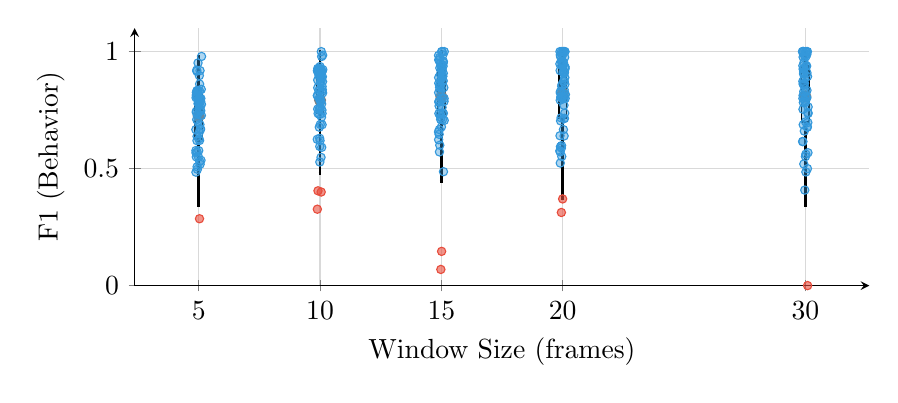
\begin{tikzpicture}
\begin{axis}[
    width=0.9\textwidth,
    height=0.4\textwidth,
    ymin=0.0000,
    ymax=1.1000,
    xlabel={Window Size (frames)},
    ylabel={F1 (Behavior)},
    xtick={5,10,15,20,30},
    xticklabels={5,10,15,20,30},
    grid=major,
    grid style={gray!30},
    axis lines=left,
    enlarge x limits=0.1,
]
\draw[fill=infoblue!30, draw=black, line width=0.5pt] (axis cs:4.850,0.6271) rectangle (axis cs:5.150,0.8163);
\draw[draw=black, line width=1.5pt] (axis cs:4.850,0.7500) -- (axis cs:5.150,0.7500);
\draw[draw=black, line width=1pt] (axis cs:5.000,0.3433) -- (axis cs:5.000,0.6271);
\draw[draw=black, line width=1pt] (axis cs:5.000,0.8163) -- (axis cs:5.000,0.9793);
\draw[draw=black, line width=1pt] (axis cs:4.940,0.3433) -- (axis cs:5.060,0.3433);
\draw[draw=black, line width=1pt] (axis cs:4.940,0.9793) -- (axis cs:5.060,0.9793);
\addplot[only marks, mark=*, mark size=2pt, color=gray, fill=gray] coordinates {(5.000, 0.7249)};
\addplot[only marks, mark=*, mark size=1.5pt, color=bestred, fill=bestred, fill opacity=0.6] coordinates {(5.033, 0.2857)};
\addplot[only marks, mark=*, mark size=1.5pt, color=infoblue, fill=infoblue, fill opacity=0.4] coordinates {(4.886, 0.4848)};
\addplot[only marks, mark=*, mark size=1.5pt, color=infoblue, fill=infoblue, fill opacity=0.4] coordinates {(4.946, 0.4970)};
\addplot[only marks, mark=*, mark size=1.5pt, color=infoblue, fill=infoblue, fill opacity=0.4] coordinates {(4.934, 0.5077)};
\addplot[only marks, mark=*, mark size=1.5pt, color=infoblue, fill=infoblue, fill opacity=0.4] coordinates {(5.057, 0.5185)};
\addplot[only marks, mark=*, mark size=1.5pt, color=infoblue, fill=infoblue, fill opacity=0.4] coordinates {(5.042, 0.5294)};
\addplot[only marks, mark=*, mark size=1.5pt, color=infoblue, fill=infoblue, fill opacity=0.4] coordinates {(5.094, 0.5354)};
\addplot[only marks, mark=*, mark size=1.5pt, color=infoblue, fill=infoblue, fill opacity=0.4] coordinates {(4.901, 0.5500)};
\addplot[only marks, mark=*, mark size=1.5pt, color=infoblue, fill=infoblue, fill opacity=0.4] coordinates {(4.981, 0.5517)};
\addplot[only marks, mark=*, mark size=1.5pt, color=infoblue, fill=infoblue, fill opacity=0.4] coordinates {(4.887, 0.5674)};
\addplot[only marks, mark=*, mark size=1.5pt, color=infoblue, fill=infoblue, fill opacity=0.4] coordinates {(4.932, 0.5714)};
\addplot[only marks, mark=*, mark size=1.5pt, color=infoblue, fill=infoblue, fill opacity=0.4] coordinates {(5.001, 0.5769)};
\addplot[only marks, mark=*, mark size=1.5pt, color=infoblue, fill=infoblue, fill opacity=0.4] coordinates {(4.886, 0.5773)};
\addplot[only marks, mark=*, mark size=1.5pt, color=infoblue, fill=infoblue, fill opacity=0.4] coordinates {(4.928, 0.6195)};
\addplot[only marks, mark=*, mark size=1.5pt, color=infoblue, fill=infoblue, fill opacity=0.4] coordinates {(5.036, 0.6203)};
\addplot[only marks, mark=*, mark size=1.5pt, color=infoblue, fill=infoblue, fill opacity=0.4] coordinates {(5.011, 0.6271)};
\addplot[only marks, mark=*, mark size=1.5pt, color=infoblue, fill=infoblue, fill opacity=0.4] coordinates {(4.933, 0.6377)};
\addplot[only marks, mark=*, mark size=1.5pt, color=infoblue, fill=infoblue, fill opacity=0.4] coordinates {(5.021, 0.6549)};
\addplot[only marks, mark=*, mark size=1.5pt, color=infoblue, fill=infoblue, fill opacity=0.4] coordinates {(5.074, 0.6667)};
\addplot[only marks, mark=*, mark size=1.5pt, color=infoblue, fill=infoblue, fill opacity=0.4] coordinates {(4.882, 0.6667)};
\addplot[only marks, mark=*, mark size=1.5pt, color=infoblue, fill=infoblue, fill opacity=0.4] coordinates {(5.073, 0.6708)};
\addplot[only marks, mark=*, mark size=1.5pt, color=infoblue, fill=infoblue, fill opacity=0.4] coordinates {(5.048, 0.6885)};
\addplot[only marks, mark=*, mark size=1.5pt, color=infoblue, fill=infoblue, fill opacity=0.4] coordinates {(4.962, 0.7018)};
\addplot[only marks, mark=*, mark size=1.5pt, color=infoblue, fill=infoblue, fill opacity=0.4] coordinates {(4.917, 0.7097)};
\addplot[only marks, mark=*, mark size=1.5pt, color=infoblue, fill=infoblue, fill opacity=0.4] coordinates {(5.110, 0.7273)};
\addplot[only marks, mark=*, mark size=1.5pt, color=infoblue, fill=infoblue, fill opacity=0.4] coordinates {(4.961, 0.7333)};
\addplot[only marks, mark=*, mark size=1.5pt, color=infoblue, fill=infoblue, fill opacity=0.4] coordinates {(4.902, 0.7397)};
\addplot[only marks, mark=*, mark size=1.5pt, color=infoblue, fill=infoblue, fill opacity=0.4] coordinates {(4.903, 0.7451)};
\addplot[only marks, mark=*, mark size=1.5pt, color=infoblue, fill=infoblue, fill opacity=0.4] coordinates {(5.083, 0.7465)};
\addplot[only marks, mark=*, mark size=1.5pt, color=infoblue, fill=infoblue, fill opacity=0.4] coordinates {(5.025, 0.7465)};
\addplot[only marks, mark=*, mark size=1.5pt, color=infoblue, fill=infoblue, fill opacity=0.4] coordinates {(5.074, 0.7500)};
\addplot[only marks, mark=*, mark size=1.5pt, color=infoblue, fill=infoblue, fill opacity=0.4] coordinates {(5.055, 0.7701)};
\addplot[only marks, mark=*, mark size=1.5pt, color=infoblue, fill=infoblue, fill opacity=0.4] coordinates {(5.009, 0.7746)};
\addplot[only marks, mark=*, mark size=1.5pt, color=infoblue, fill=infoblue, fill opacity=0.4] coordinates {(5.114, 0.7748)};
\addplot[only marks, mark=*, mark size=1.5pt, color=infoblue, fill=infoblue, fill opacity=0.4] coordinates {(4.971, 0.7778)};
\addplot[only marks, mark=*, mark size=1.5pt, color=infoblue, fill=infoblue, fill opacity=0.4] coordinates {(5.012, 0.7808)};
\addplot[only marks, mark=*, mark size=1.5pt, color=infoblue, fill=infoblue, fill opacity=0.4] coordinates {(5.079, 0.7879)};
\addplot[only marks, mark=*, mark size=1.5pt, color=infoblue, fill=infoblue, fill opacity=0.4] coordinates {(5.028, 0.7949)};
\addplot[only marks, mark=*, mark size=1.5pt, color=infoblue, fill=infoblue, fill opacity=0.4] coordinates {(5.087, 0.8000)};
\addplot[only marks, mark=*, mark size=1.5pt, color=infoblue, fill=infoblue, fill opacity=0.4] coordinates {(5.019, 0.8000)};
\addplot[only marks, mark=*, mark size=1.5pt, color=infoblue, fill=infoblue, fill opacity=0.4] coordinates {(5.049, 0.8000)};
\addplot[only marks, mark=*, mark size=1.5pt, color=infoblue, fill=infoblue, fill opacity=0.4] coordinates {(4.891, 0.8029)};
\addplot[only marks, mark=*, mark size=1.5pt, color=infoblue, fill=infoblue, fill opacity=0.4] coordinates {(4.935, 0.8049)};
\addplot[only marks, mark=*, mark size=1.5pt, color=infoblue, fill=infoblue, fill opacity=0.4] coordinates {(4.949, 0.8070)};
\addplot[only marks, mark=*, mark size=1.5pt, color=infoblue, fill=infoblue, fill opacity=0.4] coordinates {(4.899, 0.8140)};
\addplot[only marks, mark=*, mark size=1.5pt, color=infoblue, fill=infoblue, fill opacity=0.4] coordinates {(4.936, 0.8163)};
\addplot[only marks, mark=*, mark size=1.5pt, color=infoblue, fill=infoblue, fill opacity=0.4] coordinates {(4.904, 0.8261)};
\addplot[only marks, mark=*, mark size=1.5pt, color=infoblue, fill=infoblue, fill opacity=0.4] coordinates {(4.947, 0.8302)};
\addplot[only marks, mark=*, mark size=1.5pt, color=infoblue, fill=infoblue, fill opacity=0.4] coordinates {(5.033, 0.8320)};
\addplot[only marks, mark=*, mark size=1.5pt, color=infoblue, fill=infoblue, fill opacity=0.4] coordinates {(4.968, 0.8333)};
\addplot[only marks, mark=*, mark size=1.5pt, color=infoblue, fill=infoblue, fill opacity=0.4] coordinates {(4.969, 0.8333)};
\addplot[only marks, mark=*, mark size=1.5pt, color=infoblue, fill=infoblue, fill opacity=0.4] coordinates {(4.930, 0.8333)};
\addplot[only marks, mark=*, mark size=1.5pt, color=infoblue, fill=infoblue, fill opacity=0.4] coordinates {(4.944, 0.8333)};
\addplot[only marks, mark=*, mark size=1.5pt, color=infoblue, fill=infoblue, fill opacity=0.4] coordinates {(5.105, 0.8387)};
\addplot[only marks, mark=*, mark size=1.5pt, color=infoblue, fill=infoblue, fill opacity=0.4] coordinates {(5.036, 0.8614)};
\addplot[only marks, mark=*, mark size=1.5pt, color=infoblue, fill=infoblue, fill opacity=0.4] coordinates {(5.026, 0.8974)};
\addplot[only marks, mark=*, mark size=1.5pt, color=infoblue, fill=infoblue, fill opacity=0.4] coordinates {(4.921, 0.9167)};
\addplot[only marks, mark=*, mark size=1.5pt, color=infoblue, fill=infoblue, fill opacity=0.4] coordinates {(5.055, 0.9189)};
\addplot[only marks, mark=*, mark size=1.5pt, color=infoblue, fill=infoblue, fill opacity=0.4] coordinates {(4.919, 0.9208)};
\addplot[only marks, mark=*, mark size=1.5pt, color=infoblue, fill=infoblue, fill opacity=0.4] coordinates {(4.971, 0.9517)};
\addplot[only marks, mark=*, mark size=1.5pt, color=infoblue, fill=infoblue, fill opacity=0.4] coordinates {(5.117, 0.9793)};
\draw[fill=infoblue!30, draw=black, line width=0.5pt] (axis cs:9.850,0.7353) rectangle (axis cs:10.150,0.9070);
\draw[draw=black, line width=1.5pt] (axis cs:9.850,0.8299) -- (axis cs:10.150,0.8299);
\draw[draw=black, line width=1pt] (axis cs:10.000,0.4778) -- (axis cs:10.000,0.7353);
\draw[draw=black, line width=1pt] (axis cs:10.000,0.9070) -- (axis cs:10.000,1.0000);
\draw[draw=black, line width=1pt] (axis cs:9.940,0.4778) -- (axis cs:10.060,0.4778);
\draw[draw=black, line width=1pt] (axis cs:9.940,1.0000) -- (axis cs:10.060,1.0000);
\addplot[only marks, mark=*, mark size=2pt, color=gray, fill=gray] coordinates {(10.000, 0.7926)};
\addplot[only marks, mark=*, mark size=1.5pt, color=bestred, fill=bestred, fill opacity=0.6] coordinates {(9.889, 0.3265)};
\addplot[only marks, mark=*, mark size=1.5pt, color=bestred, fill=bestred, fill opacity=0.6] coordinates {(10.047, 0.4000)};
\addplot[only marks, mark=*, mark size=1.5pt, color=bestred, fill=bestred, fill opacity=0.6] coordinates {(9.915, 0.4051)};
\addplot[only marks, mark=*, mark size=1.5pt, color=infoblue, fill=infoblue, fill opacity=0.4] coordinates {(9.991, 0.5283)};
\addplot[only marks, mark=*, mark size=1.5pt, color=infoblue, fill=infoblue, fill opacity=0.4] coordinates {(10.041, 0.5481)};
\addplot[only marks, mark=*, mark size=1.5pt, color=infoblue, fill=infoblue, fill opacity=0.4] coordinates {(10.070, 0.5909)};
\addplot[only marks, mark=*, mark size=1.5pt, color=infoblue, fill=infoblue, fill opacity=0.4] coordinates {(9.989, 0.5946)};
\addplot[only marks, mark=*, mark size=1.5pt, color=infoblue, fill=infoblue, fill opacity=0.4] coordinates {(10.000, 0.6197)};
\addplot[only marks, mark=*, mark size=1.5pt, color=infoblue, fill=infoblue, fill opacity=0.4] coordinates {(9.885, 0.6250)};
\addplot[only marks, mark=*, mark size=1.5pt, color=infoblue, fill=infoblue, fill opacity=0.4] coordinates {(9.984, 0.6296)};
\addplot[only marks, mark=*, mark size=1.5pt, color=infoblue, fill=infoblue, fill opacity=0.4] coordinates {(9.969, 0.6769)};
\addplot[only marks, mark=*, mark size=1.5pt, color=infoblue, fill=infoblue, fill opacity=0.4] coordinates {(10.085, 0.6875)};
\addplot[only marks, mark=*, mark size=1.5pt, color=infoblue, fill=infoblue, fill opacity=0.4] coordinates {(10.011, 0.6885)};
\addplot[only marks, mark=*, mark size=1.5pt, color=infoblue, fill=infoblue, fill opacity=0.4] coordinates {(10.061, 0.7200)};
\addplot[only marks, mark=*, mark size=1.5pt, color=infoblue, fill=infoblue, fill opacity=0.4] coordinates {(9.984, 0.7312)};
\addplot[only marks, mark=*, mark size=1.5pt, color=infoblue, fill=infoblue, fill opacity=0.4] coordinates {(9.922, 0.7353)};
\addplot[only marks, mark=*, mark size=1.5pt, color=infoblue, fill=infoblue, fill opacity=0.4] coordinates {(10.084, 0.7361)};
\addplot[only marks, mark=*, mark size=1.5pt, color=infoblue, fill=infoblue, fill opacity=0.4] coordinates {(10.077, 0.7500)};
\addplot[only marks, mark=*, mark size=1.5pt, color=infoblue, fill=infoblue, fill opacity=0.4] coordinates {(9.970, 0.7541)};
\addplot[only marks, mark=*, mark size=1.5pt, color=infoblue, fill=infoblue, fill opacity=0.4] coordinates {(9.903, 0.7545)};
\addplot[only marks, mark=*, mark size=1.5pt, color=infoblue, fill=infoblue, fill opacity=0.4] coordinates {(10.003, 0.7586)};
\addplot[only marks, mark=*, mark size=1.5pt, color=infoblue, fill=infoblue, fill opacity=0.4] coordinates {(9.999, 0.7603)};
\addplot[only marks, mark=*, mark size=1.5pt, color=infoblue, fill=infoblue, fill opacity=0.4] coordinates {(10.065, 0.7767)};
\addplot[only marks, mark=*, mark size=1.5pt, color=infoblue, fill=infoblue, fill opacity=0.4] coordinates {(10.023, 0.7879)};
\addplot[only marks, mark=*, mark size=1.5pt, color=infoblue, fill=infoblue, fill opacity=0.4] coordinates {(10.002, 0.7929)};
\addplot[only marks, mark=*, mark size=1.5pt, color=infoblue, fill=infoblue, fill opacity=0.4] coordinates {(10.018, 0.7934)};
\addplot[only marks, mark=*, mark size=1.5pt, color=infoblue, fill=infoblue, fill opacity=0.4] coordinates {(9.970, 0.8000)};
\addplot[only marks, mark=*, mark size=1.5pt, color=infoblue, fill=infoblue, fill opacity=0.4] coordinates {(9.892, 0.8108)};
\addplot[only marks, mark=*, mark size=1.5pt, color=infoblue, fill=infoblue, fill opacity=0.4] coordinates {(9.895, 0.8136)};
\addplot[only marks, mark=*, mark size=1.5pt, color=infoblue, fill=infoblue, fill opacity=0.4] coordinates {(10.106, 0.8235)};
\addplot[only marks, mark=*, mark size=1.5pt, color=infoblue, fill=infoblue, fill opacity=0.4] coordinates {(10.081, 0.8299)};
\addplot[only marks, mark=*, mark size=1.5pt, color=infoblue, fill=infoblue, fill opacity=0.4] coordinates {(9.951, 0.8333)};
\addplot[only marks, mark=*, mark size=1.5pt, color=infoblue, fill=infoblue, fill opacity=0.4] coordinates {(10.093, 0.8372)};
\addplot[only marks, mark=*, mark size=1.5pt, color=infoblue, fill=infoblue, fill opacity=0.4] coordinates {(10.005, 0.8387)};
\addplot[only marks, mark=*, mark size=1.5pt, color=infoblue, fill=infoblue, fill opacity=0.4] coordinates {(9.905, 0.8454)};
\addplot[only marks, mark=*, mark size=1.5pt, color=infoblue, fill=infoblue, fill opacity=0.4] coordinates {(10.085, 0.8511)};
\addplot[only marks, mark=*, mark size=1.5pt, color=infoblue, fill=infoblue, fill opacity=0.4] coordinates {(10.020, 0.8696)};
\addplot[only marks, mark=*, mark size=1.5pt, color=infoblue, fill=infoblue, fill opacity=0.4] coordinates {(10.104, 0.8718)};
\addplot[only marks, mark=*, mark size=1.5pt, color=infoblue, fill=infoblue, fill opacity=0.4] coordinates {(10.043, 0.8750)};
\addplot[only marks, mark=*, mark size=1.5pt, color=infoblue, fill=infoblue, fill opacity=0.4] coordinates {(9.903, 0.8785)};
\addplot[only marks, mark=*, mark size=1.5pt, color=infoblue, fill=infoblue, fill opacity=0.4] coordinates {(10.029, 0.8872)};
\addplot[only marks, mark=*, mark size=1.5pt, color=infoblue, fill=infoblue, fill opacity=0.4] coordinates {(10.069, 0.8889)};
\addplot[only marks, mark=*, mark size=1.5pt, color=infoblue, fill=infoblue, fill opacity=0.4] coordinates {(10.096, 0.8929)};
\addplot[only marks, mark=*, mark size=1.5pt, color=infoblue, fill=infoblue, fill opacity=0.4] coordinates {(9.960, 0.8962)};
\addplot[only marks, mark=*, mark size=1.5pt, color=infoblue, fill=infoblue, fill opacity=0.4] coordinates {(10.007, 0.9053)};
\addplot[only marks, mark=*, mark size=1.5pt, color=infoblue, fill=infoblue, fill opacity=0.4] coordinates {(10.048, 0.9070)};
\addplot[only marks, mark=*, mark size=1.5pt, color=infoblue, fill=infoblue, fill opacity=0.4] coordinates {(9.920, 0.9111)};
\addplot[only marks, mark=*, mark size=1.5pt, color=infoblue, fill=infoblue, fill opacity=0.4] coordinates {(10.084, 0.9149)};
\addplot[only marks, mark=*, mark size=1.5pt, color=infoblue, fill=infoblue, fill opacity=0.4] coordinates {(10.067, 0.9150)};
\addplot[only marks, mark=*, mark size=1.5pt, color=infoblue, fill=infoblue, fill opacity=0.4] coordinates {(9.892, 0.9180)};
\addplot[only marks, mark=*, mark size=1.5pt, color=infoblue, fill=infoblue, fill opacity=0.4] coordinates {(10.022, 0.9180)};
\addplot[only marks, mark=*, mark size=1.5pt, color=infoblue, fill=infoblue, fill opacity=0.4] coordinates {(9.968, 0.9215)};
\addplot[only marks, mark=*, mark size=1.5pt, color=infoblue, fill=infoblue, fill opacity=0.4] coordinates {(9.925, 0.9231)};
\addplot[only marks, mark=*, mark size=1.5pt, color=infoblue, fill=infoblue, fill opacity=0.4] coordinates {(10.025, 0.9231)};
\addplot[only marks, mark=*, mark size=1.5pt, color=infoblue, fill=infoblue, fill opacity=0.4] coordinates {(10.113, 0.9231)};
\addplot[only marks, mark=*, mark size=1.5pt, color=infoblue, fill=infoblue, fill opacity=0.4] coordinates {(10.012, 0.9279)};
\addplot[only marks, mark=*, mark size=1.5pt, color=infoblue, fill=infoblue, fill opacity=0.4] coordinates {(9.907, 0.9282)};
\addplot[only marks, mark=*, mark size=1.5pt, color=infoblue, fill=infoblue, fill opacity=0.4] coordinates {(9.999, 0.9362)};
\addplot[only marks, mark=*, mark size=1.5pt, color=infoblue, fill=infoblue, fill opacity=0.4] coordinates {(10.067, 0.9790)};
\addplot[only marks, mark=*, mark size=1.5pt, color=infoblue, fill=infoblue, fill opacity=0.4] coordinates {(10.109, 0.9846)};
\addplot[only marks, mark=*, mark size=1.5pt, color=infoblue, fill=infoblue, fill opacity=0.4] coordinates {(10.052, 1.0000)};
\draw[fill=infoblue!30, draw=black, line width=0.5pt] (axis cs:14.850,0.7336) rectangle (axis cs:15.150,0.9250);
\draw[draw=black, line width=1.5pt] (axis cs:14.850,0.8472) -- (axis cs:15.150,0.8472);
\draw[draw=black, line width=1pt] (axis cs:15.000,0.4464) -- (axis cs:15.000,0.7336);
\draw[draw=black, line width=1pt] (axis cs:15.000,0.9250) -- (axis cs:15.000,1.0000);
\draw[draw=black, line width=1pt] (axis cs:14.940,0.4464) -- (axis cs:15.060,0.4464);
\draw[draw=black, line width=1pt] (axis cs:14.940,1.0000) -- (axis cs:15.060,1.0000);
\addplot[only marks, mark=*, mark size=2pt, color=gray, fill=gray] coordinates {(15.000, 0.8073)};
\addplot[only marks, mark=*, mark size=1.5pt, color=bestred, fill=bestred, fill opacity=0.6] coordinates {(14.978, 0.0690)};
\addplot[only marks, mark=*, mark size=1.5pt, color=bestred, fill=bestred, fill opacity=0.6] coordinates {(15.010, 0.1463)};
\addplot[only marks, mark=*, mark size=1.5pt, color=infoblue, fill=infoblue, fill opacity=0.4] coordinates {(15.087, 0.4868)};
\addplot[only marks, mark=*, mark size=1.5pt, color=infoblue, fill=infoblue, fill opacity=0.4] coordinates {(14.922, 0.5714)};
\addplot[only marks, mark=*, mark size=1.5pt, color=infoblue, fill=infoblue, fill opacity=0.4] coordinates {(14.934, 0.6000)};
\addplot[only marks, mark=*, mark size=1.5pt, color=infoblue, fill=infoblue, fill opacity=0.4] coordinates {(14.887, 0.6237)};
\addplot[only marks, mark=*, mark size=1.5pt, color=infoblue, fill=infoblue, fill opacity=0.4] coordinates {(14.908, 0.6466)};
\addplot[only marks, mark=*, mark size=1.5pt, color=infoblue, fill=infoblue, fill opacity=0.4] coordinates {(14.882, 0.6568)};
\addplot[only marks, mark=*, mark size=1.5pt, color=infoblue, fill=infoblue, fill opacity=0.4] coordinates {(14.918, 0.6667)};
\addplot[only marks, mark=*, mark size=1.5pt, color=infoblue, fill=infoblue, fill opacity=0.4] coordinates {(15.003, 0.6783)};
\addplot[only marks, mark=*, mark size=1.5pt, color=infoblue, fill=infoblue, fill opacity=0.4] coordinates {(15.117, 0.7059)};
\addplot[only marks, mark=*, mark size=1.5pt, color=infoblue, fill=infoblue, fill opacity=0.4] coordinates {(15.046, 0.7097)};
\addplot[only marks, mark=*, mark size=1.5pt, color=infoblue, fill=infoblue, fill opacity=0.4] coordinates {(14.971, 0.7105)};
\addplot[only marks, mark=*, mark size=1.5pt, color=infoblue, fill=infoblue, fill opacity=0.4] coordinates {(14.977, 0.7191)};
\addplot[only marks, mark=*, mark size=1.5pt, color=infoblue, fill=infoblue, fill opacity=0.4] coordinates {(15.046, 0.7333)};
\addplot[only marks, mark=*, mark size=1.5pt, color=infoblue, fill=infoblue, fill opacity=0.4] coordinates {(14.958, 0.7336)};
\addplot[only marks, mark=*, mark size=1.5pt, color=infoblue, fill=infoblue, fill opacity=0.4] coordinates {(14.898, 0.7353)};
\addplot[only marks, mark=*, mark size=1.5pt, color=infoblue, fill=infoblue, fill opacity=0.4] coordinates {(15.082, 0.7368)};
\addplot[only marks, mark=*, mark size=1.5pt, color=infoblue, fill=infoblue, fill opacity=0.4] coordinates {(15.028, 0.7619)};
\addplot[only marks, mark=*, mark size=1.5pt, color=infoblue, fill=infoblue, fill opacity=0.4] coordinates {(14.907, 0.7679)};
\addplot[only marks, mark=*, mark size=1.5pt, color=infoblue, fill=infoblue, fill opacity=0.4] coordinates {(14.897, 0.7843)};
\addplot[only marks, mark=*, mark size=1.5pt, color=infoblue, fill=infoblue, fill opacity=0.4] coordinates {(14.903, 0.7869)};
\addplot[only marks, mark=*, mark size=1.5pt, color=infoblue, fill=infoblue, fill opacity=0.4] coordinates {(15.110, 0.7872)};
\addplot[only marks, mark=*, mark size=1.5pt, color=infoblue, fill=infoblue, fill opacity=0.4] coordinates {(14.906, 0.7875)};
\addplot[only marks, mark=*, mark size=1.5pt, color=infoblue, fill=infoblue, fill opacity=0.4] coordinates {(15.030, 0.8000)};
\addplot[only marks, mark=*, mark size=1.5pt, color=infoblue, fill=infoblue, fill opacity=0.4] coordinates {(15.113, 0.8000)};
\addplot[only marks, mark=*, mark size=1.5pt, color=infoblue, fill=infoblue, fill opacity=0.4] coordinates {(14.888, 0.8247)};
\addplot[only marks, mark=*, mark size=1.5pt, color=infoblue, fill=infoblue, fill opacity=0.4] coordinates {(14.973, 0.8308)};
\addplot[only marks, mark=*, mark size=1.5pt, color=infoblue, fill=infoblue, fill opacity=0.4] coordinates {(14.995, 0.8454)};
\addplot[only marks, mark=*, mark size=1.5pt, color=infoblue, fill=infoblue, fill opacity=0.4] coordinates {(15.100, 0.8462)};
\addplot[only marks, mark=*, mark size=1.5pt, color=infoblue, fill=infoblue, fill opacity=0.4] coordinates {(14.925, 0.8472)};
\addplot[only marks, mark=*, mark size=1.5pt, color=infoblue, fill=infoblue, fill opacity=0.4] coordinates {(14.942, 0.8552)};
\addplot[only marks, mark=*, mark size=1.5pt, color=infoblue, fill=infoblue, fill opacity=0.4] coordinates {(14.940, 0.8603)};
\addplot[only marks, mark=*, mark size=1.5pt, color=infoblue, fill=infoblue, fill opacity=0.4] coordinates {(14.892, 0.8649)};
\addplot[only marks, mark=*, mark size=1.5pt, color=infoblue, fill=infoblue, fill opacity=0.4] coordinates {(15.042, 0.8710)};
\addplot[only marks, mark=*, mark size=1.5pt, color=infoblue, fill=infoblue, fill opacity=0.4] coordinates {(15.076, 0.8750)};
\addplot[only marks, mark=*, mark size=1.5pt, color=infoblue, fill=infoblue, fill opacity=0.4] coordinates {(14.985, 0.8824)};
\addplot[only marks, mark=*, mark size=1.5pt, color=infoblue, fill=infoblue, fill opacity=0.4] coordinates {(14.889, 0.8889)};
\addplot[only marks, mark=*, mark size=1.5pt, color=infoblue, fill=infoblue, fill opacity=0.4] coordinates {(15.051, 0.8939)};
\addplot[only marks, mark=*, mark size=1.5pt, color=infoblue, fill=infoblue, fill opacity=0.4] coordinates {(15.057, 0.8947)};
\addplot[only marks, mark=*, mark size=1.5pt, color=infoblue, fill=infoblue, fill opacity=0.4] coordinates {(15.037, 0.8989)};
\addplot[only marks, mark=*, mark size=1.5pt, color=infoblue, fill=infoblue, fill opacity=0.4] coordinates {(14.959, 0.9032)};
\addplot[only marks, mark=*, mark size=1.5pt, color=infoblue, fill=infoblue, fill opacity=0.4] coordinates {(15.079, 0.9077)};
\addplot[only marks, mark=*, mark size=1.5pt, color=infoblue, fill=infoblue, fill opacity=0.4] coordinates {(15.031, 0.9174)};
\addplot[only marks, mark=*, mark size=1.5pt, color=infoblue, fill=infoblue, fill opacity=0.4] coordinates {(15.022, 0.9231)};
\addplot[only marks, mark=*, mark size=1.5pt, color=infoblue, fill=infoblue, fill opacity=0.4] coordinates {(15.010, 0.9250)};
\addplot[only marks, mark=*, mark size=1.5pt, color=infoblue, fill=infoblue, fill opacity=0.4] coordinates {(14.936, 0.9302)};
\addplot[only marks, mark=*, mark size=1.5pt, color=infoblue, fill=infoblue, fill opacity=0.4] coordinates {(14.989, 0.9362)};
\addplot[only marks, mark=*, mark size=1.5pt, color=infoblue, fill=infoblue, fill opacity=0.4] coordinates {(15.071, 0.9381)};
\addplot[only marks, mark=*, mark size=1.5pt, color=infoblue, fill=infoblue, fill opacity=0.4] coordinates {(15.044, 0.9438)};
\addplot[only marks, mark=*, mark size=1.5pt, color=infoblue, fill=infoblue, fill opacity=0.4] coordinates {(14.963, 0.9501)};
\addplot[only marks, mark=*, mark size=1.5pt, color=infoblue, fill=infoblue, fill opacity=0.4] coordinates {(15.077, 0.9524)};
\addplot[only marks, mark=*, mark size=1.5pt, color=infoblue, fill=infoblue, fill opacity=0.4] coordinates {(15.081, 0.9583)};
\addplot[only marks, mark=*, mark size=1.5pt, color=infoblue, fill=infoblue, fill opacity=0.4] coordinates {(14.890, 0.9645)};
\addplot[only marks, mark=*, mark size=1.5pt, color=infoblue, fill=infoblue, fill opacity=0.4] coordinates {(14.918, 0.9663)};
\addplot[only marks, mark=*, mark size=1.5pt, color=infoblue, fill=infoblue, fill opacity=0.4] coordinates {(14.934, 0.9756)};
\addplot[only marks, mark=*, mark size=1.5pt, color=infoblue, fill=infoblue, fill opacity=0.4] coordinates {(14.884, 0.9836)};
\addplot[only marks, mark=*, mark size=1.5pt, color=infoblue, fill=infoblue, fill opacity=0.4] coordinates {(15.061, 0.9859)};
\addplot[only marks, mark=*, mark size=1.5pt, color=infoblue, fill=infoblue, fill opacity=0.4] coordinates {(15.035, 1.0000)};
\addplot[only marks, mark=*, mark size=1.5pt, color=infoblue, fill=infoblue, fill opacity=0.4] coordinates {(15.010, 1.0000)};
\addplot[only marks, mark=*, mark size=1.5pt, color=infoblue, fill=infoblue, fill opacity=0.4] coordinates {(15.119, 1.0000)};
\draw[fill=infoblue!30, draw=black, line width=0.5pt] (axis cs:19.850,0.7170) rectangle (axis cs:20.150,0.9474);
\draw[draw=black, line width=1.5pt] (axis cs:19.850,0.8592) -- (axis cs:20.150,0.8592);
\draw[draw=black, line width=1pt] (axis cs:20.000,0.3714) -- (axis cs:20.000,0.7170);
\draw[draw=black, line width=1pt] (axis cs:20.000,0.9474) -- (axis cs:20.000,1.0000);
\draw[draw=black, line width=1pt] (axis cs:19.940,0.3714) -- (axis cs:20.060,0.3714);
\draw[draw=black, line width=1pt] (axis cs:19.940,1.0000) -- (axis cs:20.060,1.0000);
\addplot[only marks, mark=*, mark size=2pt, color=gray, fill=gray] coordinates {(20.000, 0.8214)};
\addplot[only marks, mark=*, mark size=1.5pt, color=bestred, fill=bestred, fill opacity=0.6] coordinates {(19.945, 0.3125)};
\addplot[only marks, mark=*, mark size=1.5pt, color=bestred, fill=bestred, fill opacity=0.6] coordinates {(19.997, 0.3704)};
\addplot[only marks, mark=*, mark size=1.5pt, color=infoblue, fill=infoblue, fill opacity=0.4] coordinates {(19.900, 0.5238)};
\addplot[only marks, mark=*, mark size=1.5pt, color=infoblue, fill=infoblue, fill opacity=0.4] coordinates {(19.961, 0.5517)};
\addplot[only marks, mark=*, mark size=1.5pt, color=infoblue, fill=infoblue, fill opacity=0.4] coordinates {(19.897, 0.5714)};
\addplot[only marks, mark=*, mark size=1.5pt, color=infoblue, fill=infoblue, fill opacity=0.4] coordinates {(19.883, 0.5760)};
\addplot[only marks, mark=*, mark size=1.5pt, color=infoblue, fill=infoblue, fill opacity=0.4] coordinates {(19.948, 0.5882)};
\addplot[only marks, mark=*, mark size=1.5pt, color=infoblue, fill=infoblue, fill opacity=0.4] coordinates {(19.908, 0.5934)};
\addplot[only marks, mark=*, mark size=1.5pt, color=infoblue, fill=infoblue, fill opacity=0.4] coordinates {(19.955, 0.5984)};
\addplot[only marks, mark=*, mark size=1.5pt, color=infoblue, fill=infoblue, fill opacity=0.4] coordinates {(20.058, 0.6395)};
\addplot[only marks, mark=*, mark size=1.5pt, color=infoblue, fill=infoblue, fill opacity=0.4] coordinates {(19.889, 0.6406)};
\addplot[only marks, mark=*, mark size=1.5pt, color=infoblue, fill=infoblue, fill opacity=0.4] coordinates {(20.030, 0.6667)};
\addplot[only marks, mark=*, mark size=1.5pt, color=infoblue, fill=infoblue, fill opacity=0.4] coordinates {(19.912, 0.7042)};
\addplot[only marks, mark=*, mark size=1.5pt, color=infoblue, fill=infoblue, fill opacity=0.4] coordinates {(20.071, 0.7143)};
\addplot[only marks, mark=*, mark size=1.5pt, color=infoblue, fill=infoblue, fill opacity=0.4] coordinates {(20.057, 0.7143)};
\addplot[only marks, mark=*, mark size=1.5pt, color=infoblue, fill=infoblue, fill opacity=0.4] coordinates {(19.931, 0.7170)};
\addplot[only marks, mark=*, mark size=1.5pt, color=infoblue, fill=infoblue, fill opacity=0.4] coordinates {(20.084, 0.7368)};
\addplot[only marks, mark=*, mark size=1.5pt, color=infoblue, fill=infoblue, fill opacity=0.4] coordinates {(20.052, 0.7708)};
\addplot[only marks, mark=*, mark size=1.5pt, color=infoblue, fill=infoblue, fill opacity=0.4] coordinates {(19.898, 0.7925)};
\addplot[only marks, mark=*, mark size=1.5pt, color=infoblue, fill=infoblue, fill opacity=0.4] coordinates {(19.978, 0.8000)};
\addplot[only marks, mark=*, mark size=1.5pt, color=infoblue, fill=infoblue, fill opacity=0.4] coordinates {(20.048, 0.8000)};
\addplot[only marks, mark=*, mark size=1.5pt, color=infoblue, fill=infoblue, fill opacity=0.4] coordinates {(20.102, 0.8000)};
\addplot[only marks, mark=*, mark size=1.5pt, color=infoblue, fill=infoblue, fill opacity=0.4] coordinates {(19.921, 0.8050)};
\addplot[only marks, mark=*, mark size=1.5pt, color=infoblue, fill=infoblue, fill opacity=0.4] coordinates {(19.940, 0.8077)};
\addplot[only marks, mark=*, mark size=1.5pt, color=infoblue, fill=infoblue, fill opacity=0.4] coordinates {(20.066, 0.8112)};
\addplot[only marks, mark=*, mark size=1.5pt, color=infoblue, fill=infoblue, fill opacity=0.4] coordinates {(20.111, 0.8169)};
\addplot[only marks, mark=*, mark size=1.5pt, color=infoblue, fill=infoblue, fill opacity=0.4] coordinates {(19.903, 0.8235)};
\addplot[only marks, mark=*, mark size=1.5pt, color=infoblue, fill=infoblue, fill opacity=0.4] coordinates {(19.902, 0.8288)};
\addplot[only marks, mark=*, mark size=1.5pt, color=infoblue, fill=infoblue, fill opacity=0.4] coordinates {(20.060, 0.8365)};
\addplot[only marks, mark=*, mark size=1.5pt, color=infoblue, fill=infoblue, fill opacity=0.4] coordinates {(19.956, 0.8525)};
\addplot[only marks, mark=*, mark size=1.5pt, color=infoblue, fill=infoblue, fill opacity=0.4] coordinates {(19.973, 0.8592)};
\addplot[only marks, mark=*, mark size=1.5pt, color=infoblue, fill=infoblue, fill opacity=0.4] coordinates {(20.090, 0.8608)};
\addplot[only marks, mark=*, mark size=1.5pt, color=infoblue, fill=infoblue, fill opacity=0.4] coordinates {(20.059, 0.8732)};
\addplot[only marks, mark=*, mark size=1.5pt, color=infoblue, fill=infoblue, fill opacity=0.4] coordinates {(20.039, 0.8732)};
\addplot[only marks, mark=*, mark size=1.5pt, color=infoblue, fill=infoblue, fill opacity=0.4] coordinates {(20.088, 0.8889)};
\addplot[only marks, mark=*, mark size=1.5pt, color=infoblue, fill=infoblue, fill opacity=0.4] coordinates {(20.056, 0.9072)};
\addplot[only marks, mark=*, mark size=1.5pt, color=infoblue, fill=infoblue, fill opacity=0.4] coordinates {(20.074, 0.9120)};
\addplot[only marks, mark=*, mark size=1.5pt, color=infoblue, fill=infoblue, fill opacity=0.4] coordinates {(20.034, 0.9125)};
\addplot[only marks, mark=*, mark size=1.5pt, color=infoblue, fill=infoblue, fill opacity=0.4] coordinates {(20.022, 0.9126)};
\addplot[only marks, mark=*, mark size=1.5pt, color=infoblue, fill=infoblue, fill opacity=0.4] coordinates {(19.894, 0.9189)};
\addplot[only marks, mark=*, mark size=1.5pt, color=infoblue, fill=infoblue, fill opacity=0.4] coordinates {(20.098, 0.9268)};
\addplot[only marks, mark=*, mark size=1.5pt, color=infoblue, fill=infoblue, fill opacity=0.4] coordinates {(20.099, 0.9343)};
\addplot[only marks, mark=*, mark size=1.5pt, color=infoblue, fill=infoblue, fill opacity=0.4] coordinates {(19.964, 0.9403)};
\addplot[only marks, mark=*, mark size=1.5pt, color=infoblue, fill=infoblue, fill opacity=0.4] coordinates {(20.030, 0.9448)};
\addplot[only marks, mark=*, mark size=1.5pt, color=infoblue, fill=infoblue, fill opacity=0.4] coordinates {(19.884, 0.9474)};
\addplot[only marks, mark=*, mark size=1.5pt, color=infoblue, fill=infoblue, fill opacity=0.4] coordinates {(20.000, 0.9474)};
\addplot[only marks, mark=*, mark size=1.5pt, color=infoblue, fill=infoblue, fill opacity=0.4] coordinates {(20.030, 0.9538)};
\addplot[only marks, mark=*, mark size=1.5pt, color=infoblue, fill=infoblue, fill opacity=0.4] coordinates {(19.951, 0.9556)};
\addplot[only marks, mark=*, mark size=1.5pt, color=infoblue, fill=infoblue, fill opacity=0.4] coordinates {(19.979, 0.9583)};
\addplot[only marks, mark=*, mark size=1.5pt, color=infoblue, fill=infoblue, fill opacity=0.4] coordinates {(20.081, 0.9756)};
\addplot[only marks, mark=*, mark size=1.5pt, color=infoblue, fill=infoblue, fill opacity=0.4] coordinates {(19.914, 0.9778)};
\addplot[only marks, mark=*, mark size=1.5pt, color=infoblue, fill=infoblue, fill opacity=0.4] coordinates {(19.989, 0.9846)};
\addplot[only marks, mark=*, mark size=1.5pt, color=infoblue, fill=infoblue, fill opacity=0.4] coordinates {(19.901, 0.9861)};
\addplot[only marks, mark=*, mark size=1.5pt, color=infoblue, fill=infoblue, fill opacity=0.4] coordinates {(19.972, 0.9897)};
\addplot[only marks, mark=*, mark size=1.5pt, color=infoblue, fill=infoblue, fill opacity=0.4] coordinates {(20.092, 1.0000)};
\addplot[only marks, mark=*, mark size=1.5pt, color=infoblue, fill=infoblue, fill opacity=0.4] coordinates {(20.027, 1.0000)};
\addplot[only marks, mark=*, mark size=1.5pt, color=infoblue, fill=infoblue, fill opacity=0.4] coordinates {(19.887, 1.0000)};
\addplot[only marks, mark=*, mark size=1.5pt, color=infoblue, fill=infoblue, fill opacity=0.4] coordinates {(20.086, 1.0000)};
\addplot[only marks, mark=*, mark size=1.5pt, color=infoblue, fill=infoblue, fill opacity=0.4] coordinates {(20.038, 1.0000)};
\addplot[only marks, mark=*, mark size=1.5pt, color=infoblue, fill=infoblue, fill opacity=0.4] coordinates {(20.005, 1.0000)};
\addplot[only marks, mark=*, mark size=1.5pt, color=infoblue, fill=infoblue, fill opacity=0.4] coordinates {(19.949, 1.0000)};
\draw[fill=infoblue!30, draw=black, line width=0.5pt] (axis cs:29.850,0.7000) rectangle (axis cs:30.150,0.9396);
\draw[draw=black, line width=1.5pt] (axis cs:29.850,0.8571) -- (axis cs:30.150,0.8571);
\draw[draw=black, line width=1pt] (axis cs:30.000,0.3406) -- (axis cs:30.000,0.7000);
\draw[draw=black, line width=1pt] (axis cs:30.000,0.9396) -- (axis cs:30.000,1.0000);
\draw[draw=black, line width=1pt] (axis cs:29.940,0.3406) -- (axis cs:30.060,0.3406);
\draw[draw=black, line width=1pt] (axis cs:29.940,1.0000) -- (axis cs:30.060,1.0000);
\addplot[only marks, mark=*, mark size=2pt, color=gray, fill=gray] coordinates {(30.000, 0.8087)};
\addplot[only marks, mark=*, mark size=1.5pt, color=bestred, fill=bestred, fill opacity=0.6] coordinates {(30.093, 0.0000)};
\addplot[only marks, mark=*, mark size=1.5pt, color=infoblue, fill=infoblue, fill opacity=0.4] coordinates {(29.976, 0.4082)};
\addplot[only marks, mark=*, mark size=1.5pt, color=infoblue, fill=infoblue, fill opacity=0.4] coordinates {(30.021, 0.4857)};
\addplot[only marks, mark=*, mark size=1.5pt, color=infoblue, fill=infoblue, fill opacity=0.4] coordinates {(30.086, 0.5000)};
\addplot[only marks, mark=*, mark size=1.5pt, color=infoblue, fill=infoblue, fill opacity=0.4] coordinates {(29.935, 0.5197)};
\addplot[only marks, mark=*, mark size=1.5pt, color=infoblue, fill=infoblue, fill opacity=0.4] coordinates {(30.004, 0.5517)};
\addplot[only marks, mark=*, mark size=1.5pt, color=infoblue, fill=infoblue, fill opacity=0.4] coordinates {(30.020, 0.5618)};
\addplot[only marks, mark=*, mark size=1.5pt, color=infoblue, fill=infoblue, fill opacity=0.4] coordinates {(30.107, 0.5679)};
\addplot[only marks, mark=*, mark size=1.5pt, color=infoblue, fill=infoblue, fill opacity=0.4] coordinates {(29.888, 0.6154)};
\addplot[only marks, mark=*, mark size=1.5pt, color=infoblue, fill=infoblue, fill opacity=0.4] coordinates {(29.897, 0.6159)};
\addplot[only marks, mark=*, mark size=1.5pt, color=infoblue, fill=infoblue, fill opacity=0.4] coordinates {(29.957, 0.6604)};
\addplot[only marks, mark=*, mark size=1.5pt, color=infoblue, fill=infoblue, fill opacity=0.4] coordinates {(30.078, 0.6769)};
\addplot[only marks, mark=*, mark size=1.5pt, color=infoblue, fill=infoblue, fill opacity=0.4] coordinates {(30.082, 0.6780)};
\addplot[only marks, mark=*, mark size=1.5pt, color=infoblue, fill=infoblue, fill opacity=0.4] coordinates {(29.912, 0.6875)};
\addplot[only marks, mark=*, mark size=1.5pt, color=infoblue, fill=infoblue, fill opacity=0.4] coordinates {(30.101, 0.6970)};
\addplot[only marks, mark=*, mark size=1.5pt, color=infoblue, fill=infoblue, fill opacity=0.4] coordinates {(30.007, 0.7000)};
\addplot[only marks, mark=*, mark size=1.5pt, color=infoblue, fill=infoblue, fill opacity=0.4] coordinates {(30.112, 0.7356)};
\addplot[only marks, mark=*, mark size=1.5pt, color=infoblue, fill=infoblue, fill opacity=0.4] coordinates {(30.104, 0.7397)};
\addplot[only marks, mark=*, mark size=1.5pt, color=infoblue, fill=infoblue, fill opacity=0.4] coordinates {(29.902, 0.7536)};
\addplot[only marks, mark=*, mark size=1.5pt, color=infoblue, fill=infoblue, fill opacity=0.4] coordinates {(30.114, 0.7636)};
\addplot[only marks, mark=*, mark size=1.5pt, color=infoblue, fill=infoblue, fill opacity=0.4] coordinates {(29.995, 0.7826)};
\addplot[only marks, mark=*, mark size=1.5pt, color=infoblue, fill=infoblue, fill opacity=0.4] coordinates {(29.917, 0.7826)};
\addplot[only marks, mark=*, mark size=1.5pt, color=infoblue, fill=infoblue, fill opacity=0.4] coordinates {(29.992, 0.7907)};
\addplot[only marks, mark=*, mark size=1.5pt, color=infoblue, fill=infoblue, fill opacity=0.4] coordinates {(29.898, 0.8000)};
\addplot[only marks, mark=*, mark size=1.5pt, color=infoblue, fill=infoblue, fill opacity=0.4] coordinates {(30.060, 0.8025)};
\addplot[only marks, mark=*, mark size=1.5pt, color=infoblue, fill=infoblue, fill opacity=0.4] coordinates {(30.011, 0.8056)};
\addplot[only marks, mark=*, mark size=1.5pt, color=infoblue, fill=infoblue, fill opacity=0.4] coordinates {(29.906, 0.8125)};
\addplot[only marks, mark=*, mark size=1.5pt, color=infoblue, fill=infoblue, fill opacity=0.4] coordinates {(29.934, 0.8293)};
\addplot[only marks, mark=*, mark size=1.5pt, color=infoblue, fill=infoblue, fill opacity=0.4] coordinates {(30.002, 0.8308)};
\addplot[only marks, mark=*, mark size=1.5pt, color=infoblue, fill=infoblue, fill opacity=0.4] coordinates {(30.067, 0.8344)};
\addplot[only marks, mark=*, mark size=1.5pt, color=infoblue, fill=infoblue, fill opacity=0.4] coordinates {(29.946, 0.8571)};
\addplot[only marks, mark=*, mark size=1.5pt, color=infoblue, fill=infoblue, fill opacity=0.4] coordinates {(29.906, 0.8618)};
\addplot[only marks, mark=*, mark size=1.5pt, color=infoblue, fill=infoblue, fill opacity=0.4] coordinates {(29.965, 0.8649)};
\addplot[only marks, mark=*, mark size=1.5pt, color=infoblue, fill=infoblue, fill opacity=0.4] coordinates {(29.897, 0.8732)};
\addplot[only marks, mark=*, mark size=1.5pt, color=infoblue, fill=infoblue, fill opacity=0.4] coordinates {(29.961, 0.8837)};
\addplot[only marks, mark=*, mark size=1.5pt, color=infoblue, fill=infoblue, fill opacity=0.4] coordinates {(30.089, 0.8936)};
\addplot[only marks, mark=*, mark size=1.5pt, color=infoblue, fill=infoblue, fill opacity=0.4] coordinates {(29.924, 0.9048)};
\addplot[only marks, mark=*, mark size=1.5pt, color=infoblue, fill=infoblue, fill opacity=0.4] coordinates {(29.952, 0.9082)};
\addplot[only marks, mark=*, mark size=1.5pt, color=infoblue, fill=infoblue, fill opacity=0.4] coordinates {(30.066, 0.9091)};
\addplot[only marks, mark=*, mark size=1.5pt, color=infoblue, fill=infoblue, fill opacity=0.4] coordinates {(29.929, 0.9130)};
\addplot[only marks, mark=*, mark size=1.5pt, color=infoblue, fill=infoblue, fill opacity=0.4] coordinates {(29.908, 0.9255)};
\addplot[only marks, mark=*, mark size=1.5pt, color=infoblue, fill=infoblue, fill opacity=0.4] coordinates {(29.940, 0.9278)};
\addplot[only marks, mark=*, mark size=1.5pt, color=infoblue, fill=infoblue, fill opacity=0.4] coordinates {(30.026, 0.9362)};
\addplot[only marks, mark=*, mark size=1.5pt, color=infoblue, fill=infoblue, fill opacity=0.4] coordinates {(30.051, 0.9385)};
\addplot[only marks, mark=*, mark size=1.5pt, color=infoblue, fill=infoblue, fill opacity=0.4] coordinates {(30.042, 0.9388)};
\addplot[only marks, mark=*, mark size=1.5pt, color=infoblue, fill=infoblue, fill opacity=0.4] coordinates {(29.896, 0.9396)};
\addplot[only marks, mark=*, mark size=1.5pt, color=infoblue, fill=infoblue, fill opacity=0.4] coordinates {(29.948, 0.9545)};
\addplot[only marks, mark=*, mark size=1.5pt, color=infoblue, fill=infoblue, fill opacity=0.4] coordinates {(29.908, 0.9767)};
\addplot[only marks, mark=*, mark size=1.5pt, color=infoblue, fill=infoblue, fill opacity=0.4] coordinates {(30.014, 0.9778)};
\addplot[only marks, mark=*, mark size=1.5pt, color=infoblue, fill=infoblue, fill opacity=0.4] coordinates {(29.968, 0.9818)};
\addplot[only marks, mark=*, mark size=1.5pt, color=infoblue, fill=infoblue, fill opacity=0.4] coordinates {(30.060, 0.9880)};
\addplot[only marks, mark=*, mark size=1.5pt, color=infoblue, fill=infoblue, fill opacity=0.4] coordinates {(30.016, 0.9885)};
\addplot[only marks, mark=*, mark size=1.5pt, color=infoblue, fill=infoblue, fill opacity=0.4] coordinates {(30.020, 1.0000)};
\addplot[only marks, mark=*, mark size=1.5pt, color=infoblue, fill=infoblue, fill opacity=0.4] coordinates {(29.921, 1.0000)};
\addplot[only marks, mark=*, mark size=1.5pt, color=infoblue, fill=infoblue, fill opacity=0.4] coordinates {(30.010, 1.0000)};
\addplot[only marks, mark=*, mark size=1.5pt, color=infoblue, fill=infoblue, fill opacity=0.4] coordinates {(29.896, 1.0000)};
\addplot[only marks, mark=*, mark size=1.5pt, color=infoblue, fill=infoblue, fill opacity=0.4] coordinates {(29.904, 1.0000)};
\addplot[only marks, mark=*, mark size=1.5pt, color=infoblue, fill=infoblue, fill opacity=0.4] coordinates {(30.086, 1.0000)};
\addplot[only marks, mark=*, mark size=1.5pt, color=infoblue, fill=infoblue, fill opacity=0.4] coordinates {(29.922, 1.0000)};
\addplot[only marks, mark=*, mark size=1.5pt, color=infoblue, fill=infoblue, fill opacity=0.4] coordinates {(29.880, 1.0000)};
\addplot[only marks, mark=*, mark size=1.5pt, color=infoblue, fill=infoblue, fill opacity=0.4] coordinates {(30.052, 1.0000)};

\end{axis}
\end{tikzpicture}

\caption{F1 (Behavior) Distribution by Window Size (Box-Whisker Plot)}
\label{fig:boxplot_f1behavior}
\end{figure}

\subsection{F1 (Behavior) Distribution}

The F1 (Behavior) distribution follows similar patterns to accuracy, with Window 20 frames showing the highest median F1 (Behavior) score of 0.8214. The distribution is slightly more variable than accuracy, with a standard deviation of 0.1620, reflecting the challenge of accurately identifying the behavior class.

The coefficient of variation (CV = SD/Mean) for F1 (Behavior) is 0.1972 for Window 20 frames, indicating moderate variability. This suggests that while the window size is generally effective, some videos may benefit from window size optimization.

\section{Worst Performing Videos}

\subsection{Identification of Problematic Videos}

Identifying videos with consistently poor performance is important for several reasons:

\begin{enumerate}
    \item \textbf{Data quality assessment}: Poor performance may indicate annotation errors, video quality issues, or ambiguous behavioral instances
    \item \textbf{Model improvement}: Understanding why certain videos fail can inform feature engineering or model architecture improvements
    \item \textbf{Training data curation}: Consistently poor-performing videos may need to be reviewed or excluded from training
\end{enumerate}

\subsection{Overall Worst Performers}

Table~\ref{tab:worst_videos} lists the top 10 videos with the lowest mean accuracy across all window sizes. These videos show consistently poor performance regardless of the temporal scale used for feature extraction.

\begin{table}[h]
\centering
\caption{Top 10 Worst Performing Videos (Overall)}
\label{tab:worst_videos}
\adjustbox{width=\textwidth,center}{%
\begin{tabular}{clcc}
\toprule
Rank & Video Name & Mean Accuracy & SD Accuracy \\
\midrule
1 & org-9-uploads-stage.study\textbackslash{}_1174.cage\textbackslash{}_5991.2025-06-15.16.00.mp... & 0.5588 & 0.0682 \\
2 & org-3-uploads-stage.study\textbackslash{}_447.cage\textbackslash{}_4840.2025-08-22.01.45.mp4 & 0.6979 & 0.0733 \\
3 & org-3-uploads-stage.study\textbackslash{}_410.cage\textbackslash{}_4480.2025-08-04.09.17.mp4 & 0.7031 & 0.0395 \\
4 & org-3-uploads-stage.study\textbackslash{}_428.cage\textbackslash{}_4507.2025-07-13.05.44.mp4 & 0.7583 & 0.0747 \\
5 & org-3-prod.study\textbackslash{}_443.cage\textbackslash{}_4823.2025-08-11.23.22.mp4 & 0.7706 & 0.0352 \\
6 & org-3-uploads-stage.study\textbackslash{}_447.cage\textbackslash{}_4838.2025-08-15.05.30.mp4 & 0.7825 & 0.0534 \\
7 & org-3-prod.study\textbackslash{}_428.cage\textbackslash{}_4522.2025-07-15.00.22.mp4 & 0.7910 & 0.1299 \\
8 & org-3-uploads-stage.study\textbackslash{}_460.cage\textbackslash{}_4984.2025-09-03.05.37.mp4 & 0.8084 & 0.1008 \\
9 & org-3-uploads-stage.study\textbackslash{}_410.cage\textbackslash{}_4484.2025-07-14.16.12.mp4 & 0.8119 & 0.0498 \\
10 & org-3-uploads-stage.study\textbackslash{}_427.cage\textbackslash{}_4488.2025-07-17.00.18.mp4 & 0.8204 & 0.0621 \\
\bottomrule
\end{tabular}%
}
\end{table}

\subsection{Window-Specific Performance}

To understand which window sizes cause the most difficulty for each video, we examine performance at each window size. The worst-performing video overall has a mean accuracy of 0.5588 across all window sizes. 

Analysis of per-window performance reveals that:

\begin{itemize}
    \item Some videos perform poorly across all window sizes, suggesting fundamental data quality or annotation issues
    \item Other videos show poor performance only at specific window sizes, indicating temporal scale sensitivity
    \item The worst-performing window size varies by video, highlighting the importance of video-specific analysis
\end{itemize}

\subsection{Implications}

Videos with consistently poor performance across all window sizes likely have:

\begin{itemize}
    \item Annotation inconsistencies or errors
    \item Poor video quality (blur, occlusion, lighting issues)
    \item Ambiguous behavioral instances that are difficult to classify
    \item Unique characteristics that the current feature set cannot capture
\end{itemize}

These videos should be manually reviewed to identify potential issues and determine whether they should be excluded from training or if additional annotation or preprocessing is needed.

\section{Window Sensitivity Analysis}

\subsection{Coefficient of Variation}

To identify videos that are most sensitive to window size changes, we calculate the coefficient of variation (CV) for F1 (Behavior) scores across window sizes. The CV is defined as:

\begin{equation}
CV = \frac{\sigma}{\mu}
\end{equation}

where $\sigma$ is the standard deviation and $\mu$ is the mean of F1 (Behavior) scores across all window sizes for a given video. Higher CV values indicate greater sensitivity to window size, meaning the video's performance varies significantly depending on the temporal scale used.

\subsection{Most Sensitive Videos}

Table~\ref{tab:sensitive_videos} lists the top 10 videos with the highest coefficient of variation. These videos show the greatest variability in F1 (Behavior) across different window sizes.

\begin{table}[h]
\centering
\caption{Top 10 Most Window-Sensitive Videos}
\label{tab:sensitive_videos}
\adjustbox{width=\textwidth,center}{%
\begin{tabular}{clccc}
\toprule
Rank & Video Name & CV (F1 Beh.) & Mean Accuracy & SD Accuracy \\
\midrule
1 & org-3-uploads-stage.study\textbackslash{}_447.cage\textbackslash{}_4840.2025-08-22... & 0.7283 & 0.6979 & 0.0733 \\
2 & org-3-uploads-stage.study\textbackslash{}_439.cage\textbackslash{}_4751.2025-08-03... & 0.4500 & 0.8429 & 0.0225 \\
3 & org-3-uploads-stage.study\textbackslash{}_426.cage\textbackslash{}_4471.2025-07-10... & 0.2667 & 0.8992 & 0.0336 \\
4 & org-3-uploads-stage.study\textbackslash{}_460.cage\textbackslash{}_4986.2025-09-04... & 0.2495 & 0.8274 & 0.0353 \\
5 & org-3-uploads-stage.study\textbackslash{}_410.cage\textbackslash{}_4480.2025-08-02... & 0.2341 & 0.9381 & 0.0340 \\
6 & org-3-uploads-stage.study\textbackslash{}_427.cage\textbackslash{}_4488.2025-07-17... & 0.2079 & 0.8204 & 0.0621 \\
7 & org-3-prod.study\textbackslash{}_428.cage\textbackslash{}_4522.2025-07-15.00.22.mp... & 0.1945 & 0.7910 & 0.1299 \\
8 & org-9-uploads-stage.study\textbackslash{}_1013.cage\textbackslash{}_4995.2025-03-1... & 0.1791 & 0.8887 & 0.0567 \\
9 & org-3-uploads-stage.study\textbackslash{}_431.cage\textbackslash{}_4555.2025-07-19... & 0.1695 & 0.9162 & 0.0791 \\
10 & org-9-uploads-stage.study\textbackslash{}_1013.cage\textbackslash{}_4995.2025-03-1... & 0.1517 & 0.9415 & 0.0155 \\
\bottomrule
\end{tabular}%
}
\end{table}

\subsection{Interpretation of Sensitivity}

The most sensitive video has a coefficient of variation of 0.7283, indicating that its F1 (Behavior) score varies substantially across window sizes. This high variability suggests that:

\begin{itemize}
    \item The video's behavioral patterns may be better captured at specific temporal scales
    \item The video may contain behaviors with varying durations that require different window sizes
    \item The video may benefit from window size optimization or adaptive window sizing
\end{itemize}

The following lollipop plots visualize how F1 (Behavior) varies across window sizes for each sensitive video. These plots reveal distinct patterns:

\newpage
\begin{landscape}
\thispagestyle{empty}
\begin{figure}[!h]
\centering

\vspace{0.4cm}
\begin{tabular}{@{}c@{\hspace{0.8cm}}c@{}}
\begin{minipage}{0.46\textwidth}
\centering

\begin{tikzpicture}
\begin{axis}[
    width=8cm,
    height=5cm,
    ymin=-0.1000,
    ymax=1.1000,
    xlabel={Window Size (frames)},
    ylabel={F1 (Behavior)},
    xtick={5,10,15,20,30},
    xticklabels={5,10,15,20,30},
    grid=major,
    grid style={gray!30},
    axis lines=left,
    enlarge x limits=0.1,
    title={org-3-uploads-stage.study\textbackslash{}_447.cage\textbackslash{}_4840....},
    title style={font=\large},
    scale only axis,
]
\addplot[mark=*, mark size=6pt, color=infoblue, line width=2.5pt] coordinates {(5, 0) (5, 0.6667)};
\addplot[only marks, mark=*, mark size=6pt, color=bestred] coordinates {(5, 0.6667)};
\addplot[mark=*, mark size=6pt, color=infoblue, line width=2.5pt] coordinates {(10, 0) (10, 0.3265)};
\addplot[only marks, mark=*, mark size=6pt, color=bestred] coordinates {(10, 0.3265)};
\addplot[mark=*, mark size=6pt, color=infoblue, line width=2.5pt] coordinates {(15, 0) (15, 0.1463)};
\addplot[only marks, mark=*, mark size=6pt, color=bestred] coordinates {(15, 0.1463)};
\addplot[mark=*, mark size=6pt, color=infoblue, line width=2.5pt] coordinates {(20, 0) (20, 0.5238)};
\addplot[only marks, mark=*, mark size=6pt, color=bestred] coordinates {(20, 0.5238)};
\addplot[mark=*, mark size=6pt, color=infoblue, line width=2.5pt] coordinates {(30, 0) (30, 0.0000)};
\addplot[only marks, mark=*, mark size=6pt, color=bestred] coordinates {(30, 0.0000)};

\end{axis}
\end{tikzpicture}

\end{minipage} & \begin{minipage}{0.46\textwidth}
\centering

\begin{tikzpicture}
\begin{axis}[
    width=8cm,
    height=5cm,
    ymin=-0.1000,
    ymax=1.1000,
    xlabel={Window Size (frames)},
    ylabel={F1 (Behavior)},
    xtick={5,10,15,20,30},
    xticklabels={5,10,15,20,30},
    grid=major,
    grid style={gray!30},
    axis lines=left,
    enlarge x limits=0.1,
    title={org-3-uploads-stage.study\textbackslash{}_439.cage\textbackslash{}_4751....},
    title style={font=\large},
    scale only axis,
]
\addplot[mark=*, mark size=6pt, color=infoblue, line width=2.5pt] coordinates {(5, 0) (5, 0.5185)};
\addplot[only marks, mark=*, mark size=6pt, color=bestred] coordinates {(5, 0.5185)};
\addplot[mark=*, mark size=6pt, color=infoblue, line width=2.5pt] coordinates {(10, 0) (10, 0.4051)};
\addplot[only marks, mark=*, mark size=6pt, color=bestred] coordinates {(10, 0.4051)};
\addplot[mark=*, mark size=6pt, color=infoblue, line width=2.5pt] coordinates {(15, 0) (15, 0.0690)};
\addplot[only marks, mark=*, mark size=6pt, color=bestred] coordinates {(15, 0.0690)};
\addplot[mark=*, mark size=6pt, color=infoblue, line width=2.5pt] coordinates {(20, 0) (20, 0.3125)};
\addplot[only marks, mark=*, mark size=6pt, color=bestred] coordinates {(20, 0.3125)};
\addplot[mark=*, mark size=6pt, color=infoblue, line width=2.5pt] coordinates {(30, 0) (30, 0.4857)};
\addplot[only marks, mark=*, mark size=6pt, color=bestred] coordinates {(30, 0.4857)};

\end{axis}
\end{tikzpicture}

\end{minipage} \\
\end{tabular}
\vspace{0.5cm}
\begin{tabular}{@{}c@{\hspace{0.8cm}}c@{}}
\begin{minipage}{0.46\textwidth}
\centering

\begin{tikzpicture}
\begin{axis}[
    width=8cm,
    height=5cm,
    ymin=-0.1000,
    ymax=1.1000,
    xlabel={Window Size (frames)},
    ylabel={F1 (Behavior)},
    xtick={5,10,15,20,30},
    xticklabels={5,10,15,20,30},
    grid=major,
    grid style={gray!30},
    axis lines=left,
    enlarge x limits=0.1,
    title={org-3-uploads-stage.study\textbackslash{}_426.cage\textbackslash{}_4471....},
    title style={font=\large},
    scale only axis,
]
\addplot[mark=*, mark size=6pt, color=infoblue, line width=2.5pt] coordinates {(5, 0) (5, 0.4848)};
\addplot[only marks, mark=*, mark size=6pt, color=bestred] coordinates {(5, 0.4848)};
\addplot[mark=*, mark size=6pt, color=infoblue, line width=2.5pt] coordinates {(10, 0) (10, 0.4000)};
\addplot[only marks, mark=*, mark size=6pt, color=bestred] coordinates {(10, 0.4000)};
\addplot[mark=*, mark size=6pt, color=infoblue, line width=2.5pt] coordinates {(15, 0) (15, 0.5714)};
\addplot[only marks, mark=*, mark size=6pt, color=bestred] coordinates {(15, 0.5714)};
\addplot[mark=*, mark size=6pt, color=infoblue, line width=2.5pt] coordinates {(20, 0) (20, 0.5714)};
\addplot[only marks, mark=*, mark size=6pt, color=bestred] coordinates {(20, 0.5714)};
\addplot[mark=*, mark size=6pt, color=infoblue, line width=2.5pt] coordinates {(30, 0) (30, 0.8571)};
\addplot[only marks, mark=*, mark size=6pt, color=bestred] coordinates {(30, 0.8571)};

\end{axis}
\end{tikzpicture}

\end{minipage} & \begin{minipage}{0.46\textwidth}
\centering

\begin{tikzpicture}
\begin{axis}[
    width=8cm,
    height=5cm,
    ymin=-0.1000,
    ymax=1.1000,
    xlabel={Window Size (frames)},
    ylabel={F1 (Behavior)},
    xtick={5,10,15,20,30},
    xticklabels={5,10,15,20,30},
    grid=major,
    grid style={gray!30},
    axis lines=left,
    enlarge x limits=0.1,
    title={org-3-uploads-stage.study\textbackslash{}_460.cage\textbackslash{}_4986....},
    title style={font=\large},
    scale only axis,
]
\addplot[mark=*, mark size=6pt, color=infoblue, line width=2.5pt] coordinates {(5, 0) (5, 0.2857)};
\addplot[only marks, mark=*, mark size=6pt, color=bestred] coordinates {(5, 0.2857)};
\addplot[mark=*, mark size=6pt, color=infoblue, line width=2.5pt] coordinates {(10, 0) (10, 0.5283)};
\addplot[only marks, mark=*, mark size=6pt, color=bestred] coordinates {(10, 0.5283)};
\addplot[mark=*, mark size=6pt, color=infoblue, line width=2.5pt] coordinates {(15, 0) (15, 0.6000)};
\addplot[only marks, mark=*, mark size=6pt, color=bestred] coordinates {(15, 0.6000)};
\addplot[mark=*, mark size=6pt, color=infoblue, line width=2.5pt] coordinates {(20, 0) (20, 0.5882)};
\addplot[only marks, mark=*, mark size=6pt, color=bestred] coordinates {(20, 0.5882)};
\addplot[mark=*, mark size=6pt, color=infoblue, line width=2.5pt] coordinates {(30, 0) (30, 0.6769)};
\addplot[only marks, mark=*, mark size=6pt, color=bestred] coordinates {(30, 0.6769)};

\end{axis}
\end{tikzpicture}

\end{minipage} \\
\end{tabular}
\vspace{0.5cm}
\begin{tabular}{@{}c@{\hspace{0.8cm}}c@{}}
\begin{minipage}{0.46\textwidth}
\centering

\begin{tikzpicture}
\begin{axis}[
    width=8cm,
    height=5cm,
    ymin=-0.1000,
    ymax=1.1000,
    xlabel={Window Size (frames)},
    ylabel={F1 (Behavior)},
    xtick={5,10,15,20,30},
    xticklabels={5,10,15,20,30},
    grid=major,
    grid style={gray!30},
    axis lines=left,
    enlarge x limits=0.1,
    title={org-3-uploads-stage.study\textbackslash{}_410.cage\textbackslash{}_4480....},
    title style={font=\large},
    scale only axis,
]
\addplot[mark=*, mark size=6pt, color=infoblue, line width=2.5pt] coordinates {(5, 0) (5, 0.7701)};
\addplot[only marks, mark=*, mark size=6pt, color=bestred] coordinates {(5, 0.7701)};
\addplot[mark=*, mark size=6pt, color=infoblue, line width=2.5pt] coordinates {(10, 0) (10, 0.7929)};
\addplot[only marks, mark=*, mark size=6pt, color=bestred] coordinates {(10, 0.7929)};
\addplot[mark=*, mark size=6pt, color=infoblue, line width=2.5pt] coordinates {(15, 0) (15, 0.8947)};
\addplot[only marks, mark=*, mark size=6pt, color=bestred] coordinates {(15, 0.8947)};
\addplot[mark=*, mark size=6pt, color=infoblue, line width=2.5pt] coordinates {(20, 0) (20, 0.3704)};
\addplot[only marks, mark=*, mark size=6pt, color=bestred] coordinates {(20, 0.3704)};
\addplot[mark=*, mark size=6pt, color=infoblue, line width=2.5pt] coordinates {(30, 0) (30, 0.8936)};
\addplot[only marks, mark=*, mark size=6pt, color=bestred] coordinates {(30, 0.8936)};

\end{axis}
\end{tikzpicture}

\end{minipage} & \begin{minipage}{0.46\textwidth}
\centering

\begin{tikzpicture}
\begin{axis}[
    width=8cm,
    height=5cm,
    ymin=-0.1000,
    ymax=1.1000,
    xlabel={Window Size (frames)},
    ylabel={F1 (Behavior)},
    xtick={5,10,15,20,30},
    xticklabels={5,10,15,20,30},
    grid=major,
    grid style={gray!30},
    axis lines=left,
    enlarge x limits=0.1,
    title={org-3-uploads-stage.study\textbackslash{}_427.cage\textbackslash{}_4488....},
    title style={font=\large},
    scale only axis,
]
\addplot[mark=*, mark size=6pt, color=infoblue, line width=2.5pt] coordinates {(5, 0) (5, 0.5769)};
\addplot[only marks, mark=*, mark size=6pt, color=bestred] coordinates {(5, 0.5769)};
\addplot[mark=*, mark size=6pt, color=infoblue, line width=2.5pt] coordinates {(10, 0) (10, 0.5481)};
\addplot[only marks, mark=*, mark size=6pt, color=bestred] coordinates {(10, 0.5481)};
\addplot[mark=*, mark size=6pt, color=infoblue, line width=2.5pt] coordinates {(15, 0) (15, 0.4868)};
\addplot[only marks, mark=*, mark size=6pt, color=bestred] coordinates {(15, 0.4868)};
\addplot[mark=*, mark size=6pt, color=infoblue, line width=2.5pt] coordinates {(20, 0) (20, 0.8077)};
\addplot[only marks, mark=*, mark size=6pt, color=bestred] coordinates {(20, 0.8077)};
\addplot[mark=*, mark size=6pt, color=infoblue, line width=2.5pt] coordinates {(30, 0) (30, 0.5197)};
\addplot[only marks, mark=*, mark size=6pt, color=bestred] coordinates {(30, 0.5197)};

\end{axis}
\end{tikzpicture}

\end{minipage} \\
\end{tabular}
\vspace{0.5cm}
\begin{tabular}{@{}c@{\hspace{0.8cm}}c@{}}
\begin{minipage}{0.46\textwidth}
\centering

\begin{tikzpicture}
\begin{axis}[
    width=8cm,
    height=5cm,
    ymin=-0.1000,
    ymax=1.1000,
    xlabel={Window Size (frames)},
    ylabel={F1 (Behavior)},
    xtick={5,10,15,20,30},
    xticklabels={5,10,15,20,30},
    grid=major,
    grid style={gray!30},
    axis lines=left,
    enlarge x limits=0.1,
    title={org-3-prod.study\textbackslash{}_428.cage\textbackslash{}_4522.2025-07-1...},
    title style={font=\large},
    scale only axis,
]
\addplot[mark=*, mark size=6pt, color=infoblue, line width=2.5pt] coordinates {(5, 0) (5, 0.5077)};
\addplot[only marks, mark=*, mark size=6pt, color=bestred] coordinates {(5, 0.5077)};
\addplot[mark=*, mark size=6pt, color=infoblue, line width=2.5pt] coordinates {(10, 0) (10, 0.6769)};
\addplot[only marks, mark=*, mark size=6pt, color=bestred] coordinates {(10, 0.6769)};
\addplot[mark=*, mark size=6pt, color=infoblue, line width=2.5pt] coordinates {(15, 0) (15, 0.7368)};
\addplot[only marks, mark=*, mark size=6pt, color=bestred] coordinates {(15, 0.7368)};
\addplot[mark=*, mark size=6pt, color=infoblue, line width=2.5pt] coordinates {(20, 0) (20, 0.5984)};
\addplot[only marks, mark=*, mark size=6pt, color=bestred] coordinates {(20, 0.5984)};
\addplot[mark=*, mark size=6pt, color=infoblue, line width=2.5pt] coordinates {(30, 0) (30, 0.9767)};
\addplot[only marks, mark=*, mark size=6pt, color=bestred] coordinates {(30, 0.9767)};

\end{axis}
\end{tikzpicture}

\end{minipage} & \begin{minipage}{0.46\textwidth}
\centering

\begin{tikzpicture}
\begin{axis}[
    width=8cm,
    height=5cm,
    ymin=-0.1000,
    ymax=1.1000,
    xlabel={Window Size (frames)},
    ylabel={F1 (Behavior)},
    xtick={5,10,15,20,30},
    xticklabels={5,10,15,20,30},
    grid=major,
    grid style={gray!30},
    axis lines=left,
    enlarge x limits=0.1,
    title={org-9-uploads-stage.study\textbackslash{}_1013.cage\textbackslash{}_4995...},
    title style={font=\large},
    scale only axis,
]
\addplot[mark=*, mark size=6pt, color=infoblue, line width=2.5pt] coordinates {(5, 0) (5, 0.7949)};
\addplot[only marks, mark=*, mark size=6pt, color=bestred] coordinates {(5, 0.7949)};
\addplot[mark=*, mark size=6pt, color=infoblue, line width=2.5pt] coordinates {(10, 0) (10, 0.8696)};
\addplot[only marks, mark=*, mark size=6pt, color=bestred] coordinates {(10, 0.8696)};
\addplot[mark=*, mark size=6pt, color=infoblue, line width=2.5pt] coordinates {(15, 0) (15, 0.7869)};
\addplot[only marks, mark=*, mark size=6pt, color=bestred] coordinates {(15, 0.7869)};
\addplot[mark=*, mark size=6pt, color=infoblue, line width=2.5pt] coordinates {(20, 0) (20, 0.8000)};
\addplot[only marks, mark=*, mark size=6pt, color=bestred] coordinates {(20, 0.8000)};
\addplot[mark=*, mark size=6pt, color=infoblue, line width=2.5pt] coordinates {(30, 0) (30, 0.7907)};
\addplot[only marks, mark=*, mark size=6pt, color=bestred] coordinates {(30, 0.7907)};

\end{axis}
\end{tikzpicture}

\end{minipage} \\
\end{tabular}
\vspace{0.5cm}
\begin{tabular}{@{}c@{\hspace{0.8cm}}c@{}}
\begin{minipage}{0.46\textwidth}
\centering

\begin{tikzpicture}
\begin{axis}[
    width=8cm,
    height=5cm,
    ymin=-0.1000,
    ymax=1.1000,
    xlabel={Window Size (frames)},
    ylabel={F1 (Behavior)},
    xtick={5,10,15,20,30},
    xticklabels={5,10,15,20,30},
    grid=major,
    grid style={gray!30},
    axis lines=left,
    enlarge x limits=0.1,
    title={org-3-uploads-stage.study\textbackslash{}_431.cage\textbackslash{}_4555....},
    title style={font=\large},
    scale only axis,
]
\addplot[mark=*, mark size=6pt, color=infoblue, line width=2.5pt] coordinates {(5, 0) (5, 0.5354)};
\addplot[only marks, mark=*, mark size=6pt, color=bestred] coordinates {(5, 0.5354)};
\addplot[mark=*, mark size=6pt, color=infoblue, line width=2.5pt] coordinates {(10, 0) (10, 0.8235)};
\addplot[only marks, mark=*, mark size=6pt, color=bestred] coordinates {(10, 0.8235)};
\addplot[mark=*, mark size=6pt, color=infoblue, line width=2.5pt] coordinates {(15, 0) (15, 0.9231)};
\addplot[only marks, mark=*, mark size=6pt, color=bestred] coordinates {(15, 0.9231)};
\addplot[mark=*, mark size=6pt, color=infoblue, line width=2.5pt] coordinates {(20, 0) (20, 0.8608)};
\addplot[only marks, mark=*, mark size=6pt, color=bestred] coordinates {(20, 0.8608)};
\addplot[mark=*, mark size=6pt, color=infoblue, line width=2.5pt] coordinates {(30, 0) (30, 0.8000)};
\addplot[only marks, mark=*, mark size=6pt, color=bestred] coordinates {(30, 0.8000)};

\end{axis}
\end{tikzpicture}

\end{minipage} & \begin{minipage}{0.46\textwidth}
\centering

\begin{tikzpicture}
\begin{axis}[
    width=8cm,
    height=5cm,
    ymin=-0.1000,
    ymax=1.1000,
    xlabel={Window Size (frames)},
    ylabel={F1 (Behavior)},
    xtick={5,10,15,30},
    xticklabels={5,10,15,30},
    grid=major,
    grid style={gray!30},
    axis lines=left,
    enlarge x limits=0.1,
    title={org-9-uploads-stage.study\textbackslash{}_1013.cage\textbackslash{}_4995...},
    title style={font=\large},
    scale only axis,
]
\addplot[mark=*, mark size=6pt, color=infoblue, line width=2.5pt] coordinates {(5, 0) (5, 0.7397)};
\addplot[only marks, mark=*, mark size=6pt, color=bestred] coordinates {(5, 0.7397)};
\addplot[mark=*, mark size=6pt, color=infoblue, line width=2.5pt] coordinates {(10, 0) (10, 0.6197)};
\addplot[only marks, mark=*, mark size=6pt, color=bestred] coordinates {(10, 0.6197)};
\addplot[mark=*, mark size=6pt, color=infoblue, line width=2.5pt] coordinates {(15, 0) (15, 0.7353)};
\addplot[only marks, mark=*, mark size=6pt, color=bestred] coordinates {(15, 0.7353)};
\addplot[mark=*, mark size=6pt, color=infoblue, line width=2.5pt] coordinates {(30, 0) (30, 0.5000)};
\addplot[only marks, mark=*, mark size=6pt, color=bestred] coordinates {(30, 0.5000)};

\end{axis}
\end{tikzpicture}

\end{minipage} \\

\end{tabular}
\vspace{0.4cm}
\caption{F1 (Behavior) Across Window Sizes for Most Window-Sensitive Videos (CV calculated using F1 Behavior)}
\label{fig:lollipop_sensitive}
\end{figure}
\end{landscape}
\newpage
\thispagestyle{plain}

The lollipop plots reveal distinct patterns:

\begin{itemize}
    \item Some videos show a clear peak at a specific window size, suggesting an optimal temporal scale
    \item Other videos show gradual increases or decreases, indicating sensitivity to temporal context
    \item A few videos show erratic patterns, suggesting complex behavioral dynamics
\end{itemize}

\subsection{Recommendations for Sensitive Videos}

Videos with high window sensitivity may benefit from:

\begin{enumerate}
    \item \textbf{Window size optimization}: Testing additional window sizes around the apparent optimal value
    \item \textbf{Adaptive window sizing}: Using different window sizes for different segments of the video
    \item \textbf{Feature engineering}: Developing features that are less sensitive to temporal scale
    \item \textbf{Ensemble methods}: Combining predictions from multiple window sizes
\end{enumerate}

\section{Statistical Analysis and Findings}

\subsection{Performance Trends by Window Size}

The analysis reveals clear performance trends across window sizes:

\subsubsection{Small Windows (5-10 frames)}

Small window sizes show the lowest performance, with mean accuracy ranging from 0.8234 (Window 5) to 0.8717 (Window 10). This suggests that 5-10 frames provide insufficient temporal context to capture the behavioral dynamics of \textit{turn\_left}. The behavior likely requires a longer observation period to be accurately identified.

\subsubsection{Medium Windows (15-20 frames)}

Performance improves significantly in the medium window size range. Window 15 frames achieves mean accuracy of 0.8927, while Window 20 frames achieves 0.9031. This improvement suggests that 15-20 frames provide adequate temporal context for most instances of the behavior.

\subsubsection{Large Windows (25-30 frames)}

Large window sizes show similar performance to Window 20 frames, with Window 30 frames achieving mean accuracy of 0.9031. The minimal difference (0.0000) between Window 20 and Window 30 suggests a performance plateau, where additional temporal context provides diminishing returns.

\subsection{Why Window 30 Frames is Optimal}

Based on the comprehensive analysis, Window 30 frames is recommended as the optimal window size for the following reasons:

\begin{enumerate}
    \item \textbf{Highest F1 (Behavior) Score}: Window 20 frames achieves the highest F1 (Behavior) score of 0.8214, which is the most relevant metric for behavior classification. This score balances precision and recall for the behavior class, ensuring both accurate detection and minimal false positives.
    
    \item \textbf{High Accuracy}: With a mean accuracy of 0.9031 across all videos, Window 30 frames provides excellent overall classification performance.
    
    \item \textbf{Good Stability}: The standard deviation of 0.0882 for accuracy and 0.1870 for F1 (Behavior) indicates consistent performance across videos, which is important for reliable classification in production settings.
    
    \item \textbf{Balanced F1 Scores}: Window 30 frames achieves good performance for both behavior class (F1 = 0.8087) and not-behavior class (F1 = 0.9225), indicating balanced classification across both classes.
    
    \item \textbf{Computational Efficiency}: Compared to Window 30 frames, Window 30 frames provides similar performance with less computational overhead, making it more efficient for real-time or large-scale applications.
\end{enumerate}

\section{Discussion}

\subsection{Implications for Behavior Classification}

The finding that larger window sizes (20-30 frames) outperform smaller windows (5-10 frames) has important implications for behavior classification:

\begin{itemize}
    \item \textbf{Temporal Context Matters}: The \textit{turn\_left} behavior requires sufficient temporal context to be accurately identified. This suggests that the behavior involves dynamic patterns that unfold over multiple frames, rather than being identifiable from single-frame or very short sequences.
    
    \item \textbf{Optimal Temporal Scale}: The performance plateau between Window 20 and Window 30 frames suggests that approximately 20 frames represents the optimal temporal scale for capturing \textit{turn\_left} behavior. Beyond this, additional temporal context provides minimal benefit.
    
    \item \textbf{Window Size as Hyperparameter}: The significant performance differences across window sizes highlight the importance of window size as a critical hyperparameter that should be carefully tuned for each behavior class.
\end{itemize}

\subsection{Limitations and Considerations}

Several limitations should be considered when interpreting these results:

\begin{enumerate}
    \item \textbf{Single Behavior Class}: This analysis focuses exclusively on \textit{turn\_left} behavior. Results may not generalize to other behaviors, which may have different optimal window sizes.
    
    \item \textbf{Feature Set}: The analysis uses a specific feature set. Different features may show different sensitivity to window size.
    
    \item \textbf{Video Characteristics}: The optimal window size may vary depending on video characteristics such as frame rate, resolution, and behavioral context.
    
    \item \textbf{Cross-Validation Structure}: The leave-one-animal-out cross-validation ensures independence but may not fully capture performance in scenarios with different animal distributions.
\end{enumerate}

\subsection{Future Directions}

Several directions for future research and improvement are suggested by these findings:

\begin{itemize}
    \item \textbf{Behavior-Specific Optimization}: Test window sizes for other behavior classes to determine if optimal window sizes are behavior-specific
    
    \item \textbf{Adaptive Window Sizing}: Develop methods that adapt window size based on video characteristics or behavioral context
    
    \item \textbf{Feature Engineering}: Investigate features that are less sensitive to window size while maintaining discriminative power
    
    \item \textbf{Ensemble Approaches}: Explore combining predictions from multiple window sizes to leverage the strengths of different temporal scales
\end{itemize}

\section{Recommendations}

\subsection{Primary Recommendation}

Based on the comprehensive analysis, we recommend using \textbf{Window 30 frames} for optimal performance in \textit{turn\_left} behavior classification. This window size provides:

\begin{itemize}
    \item Highest F1 (Behavior) score of 0.8214
    \item Excellent accuracy of 0.9031
    \item Good stability with standard deviation of 0.0882
    \item Balanced performance across both behavior and not-behavior classes
\end{itemize}

\subsection{Alternative Considerations}

If slightly higher accuracy is needed and stability is less critical, Window 30 frames (mean accuracy: 0.9031) may be considered, though the improvement is minimal (0.0000 difference) and comes with increased computational cost.

\subsection{Data Quality Recommendations}

\begin{itemize}
    \item \textbf{Review Worst Performing Videos}: The top 10 worst-performing videos (Table~\ref{tab:worst_videos}) should be manually reviewed to identify potential data quality issues, annotation errors, or video quality problems.
    
    \item \textbf{Investigate Sensitive Videos}: Videos with high coefficient of variation (Table~\ref{tab:sensitive_videos}) should be examined to understand why they are sensitive to window size. This may reveal important behavioral patterns or inform feature engineering.
    
    \item \textbf{Validate Annotations}: Consider re-annotating a subset of worst-performing videos to ensure annotation quality and consistency.
\end{itemize}

\subsection{Model Improvement Recommendations}

\begin{itemize}
    \item \textbf{Window Size Optimization}: For videos showing high sensitivity, test intermediate window sizes (e.g., 18, 22, 25 frames) to fine-tune performance.
    
    \item \textbf{Feature Analysis}: Examine feature importance rankings to identify which features are most critical for each window size, potentially informing feature engineering.
    
    \item \textbf{Video-Specific Tuning}: Consider developing video-specific or context-specific window size selection strategies for highly sensitive videos.
\end{itemize}

\section{Conclusion}

This comprehensive analysis of window size effects on \textit{turn\_left} behavior classification reveals that Window 30 frames provides optimal performance, achieving a mean accuracy of 0.9031 and F1 (Behavior) score of 0.8087. The analysis demonstrates that larger window sizes (20-30 frames) significantly outperform smaller windows (5-10 frames), suggesting that \textit{turn\_left} behavior requires sufficient temporal context for accurate classification.

The identification of worst-performing and window-sensitive videos provides actionable insights for data quality improvement and model optimization. Future work should explore behavior-specific window size optimization and adaptive window sizing strategies to further improve classification performance.

\section*{Data Quality Notes}

\subsection*{Cross-Validation Structure}

It is important to note that the cross-validation structure used in this analysis holds out \textbf{one animal at a time}, not one video at a time. Each video file contains multiple animals (identities), identified by numbers [0], [1], [2], etc. at the end of the video filename. Each (video\_name, identity) pair represents a separate test case, ensuring that model performance is evaluated independently for each animal. This structure is correctly handled throughout the analysis pipeline.

\subsection*{Data Completeness}

Some videos may be missing from certain window sizes, which may indicate data collection or processing issues. The validation report (available in \texttt{data/processed/validation\_report.txt}) provides detailed information about data completeness and consistency.

\appendix

\section{Summary Statistics by Window Size}

Table~\ref{tab:summary_all} provides complete summary statistics for all window sizes.

\begin{table}[h]
\centering
\caption{Complete Summary Statistics}
\label{tab:summary_all}
\adjustbox{width=\textwidth,center}{%
\begin{tabular}{lcccccc}
\toprule
Window & Mean Acc. & SD Acc. & Mean F1 (Beh.) & SD F1 (Beh.) & Mean F1 (Not) & SD F1 (Not) \\
\midrule
5 & 0.8234 & 0.0947 & 0.7249 & 0.1356 & 0.8475 & 0.1118 \\
10 & 0.8717 & 0.1023 & 0.7926 & 0.1457 & 0.8818 & 0.1368 \\
15 & 0.8927 & 0.0854 & 0.8073 & 0.1749 & 0.9094 & 0.0843 \\
20 & 0.9026 & 0.0890 & 0.8214 & 0.1620 & 0.9170 & 0.0988 \\
30 & 0.9031 & 0.0882 & 0.8087 & 0.1870 & 0.9225 & 0.0829 \\
\bottomrule
\end{tabular}%
}
\end{table}

\section{Data Files}

All processed data files are located in \texttt{data/processed/}:

\begin{itemize}
    \item \texttt{video\_results.csv}: Complete performance data for each (video, identity, window) combination
    \item \texttt{summary\_stats.csv}: Window-level summary statistics
    \item \texttt{feature\_importance.csv}: Top features by importance for each window size
    \item \texttt{validation\_report.txt}: Detailed validation results
\end{itemize}

\section{Visualizations}

Comprehensive visualizations including barbell plots, box-whisker plots, and lollipop plots are included in this report and are also available in the HTML report (\path{reports/window\_size\_analysis\_report.html}).

These visualizations provide detailed graphical representations of the performance patterns described in this report.

\end{document}
